\graphicspath{{Chapters/TheoryZZProduction/Figures/}}
\chapter{ZZ Production}
\label{chap:TheoryZZProduction}

\section{Introduction}

Production of pairs of \Z\ bosons, so called \intro{diboson \ZZ\ production} is a
rare process at particle colliders, but has a very striking signature
and low backgrounds. The study of diboson \ZZ\ production is of great interest
as it provides a precision test of the \sm, and unique opportunity to
probe the structure of the electroweak sector. 
The $ZZZ$ and $ZZ\gamma$ neutral triple gauge boson
couplings (nTGCs) are zero in the Standard Model, but are predicted to exist at the
level of $10^{-4}$ to $10^{-3}$ in certain new-physics
models~\cite{Ellison:1998}. Non-resonant \ZZ\ production is also the
irreducible background to \HZZ\ decays, one of key channels in Higgs boson physics
at the LHC. The CMS~\cite{CMS_Higgs:2012gu} and ATLAS~\cite{ATLAS_Higgs:2012gk}
experiments both recently reported the discovery of a new boson with mass near
125 \gev\ in the search for the Higgs boson. \HZZ\ decays were a key
search channel for this discovery, contributing a local significance of 3.6
$\sigma$ to the overall local significance of 6.0 $\sigma$ (the other
contributing channels were \Hgg\ and \HWW). Understanding non-resonant \ZZ\
production was essential for such a discovery, and continues to be important for
studying the properties of the new boson.

\section{\ZZ\ production at hadron colliders}

At hadron colliders, \qqZZ\ proceeds at tree level via $t$- and $u$-channel
quark-antiquark annihilation as shown in~\fig{theoryzz-fd-qqZZ}. Since \ZZZ\ and
\ZZg\ couplings are forbidden in the \sm\ there is no contribution from
$s$-channel $q\bar{q}$ annihilation at tree level, although contributions from
fermion loops contribute at $\mathcal{O}(10^{-4})$~\cite{Gounaris:2000dn}.
Gluon-gluon fusion processes will also
contribute via quark box diagrams, as shown in~\fig{theoryzz-fd-ggZZ}. Although
these are NNLO and are suppressed by a factor of
$\alpha_s^2$, due to the high gluon content of the proton at LHC energies they
still contribute a sizeable fraction of the total \ZZ\ production \cx\,
contributing approximately 10\%~\cite{Campbell:2011} of the \cx,
depending on the centre of mass energy and the definition of the \cx.
This is discussed in more detail below.

%% s- and u-channel Feynman diagrams for qqZZ
\begin{figure}
\centering
    \subfigure{
        \begin{fmffile}{tchan}
        \begin{fmfgraph*}(36,20)
            \fmfleft{i1,i2}
        \fmfright{o1,o2}
        \fmflabel{$u,d$}{i2}
        \fmflabel{$\bar{u},\bar{d}$}{i1}
        \fmfright{o1,o2}
        \fmflabel{$Z/\gamma^{*}$}{o1}
        \fmflabel{$Z/\gamma^{*}$}{o2}
        \fmf{fermion}{i2,v2,v1,i1}
        %\fmf{fermion}{v2,i2}
        %\fmf{fermion}{v1,i1}
        \fmf{photon}{v1,o1}
        \fmf{photon}{v2,o2}
        % uncommment this line if you want dots at the vertices
            %\fmfdotn{v}{4}
        \end{fmfgraph*}
        \end{fmffile}
    }
    \hspace{10mm}
    \subfigure{
        \begin{fmffile}{tchan2}
        \begin{fmfgraph*}(36,20)
            \fmfleft{i1,i2}
        \fmfright{o1,o2}
        \fmflabel{$u,d$}{i2}
        \fmflabel{$\bar{u},\bar{d}$}{i1}
        \fmfright{o1,o2}
        \fmflabel{$Z/\gamma^{*}$}{o1}
        \fmflabel{$Z/\gamma^{*}$}{o2}
        \fmf{fermion}{i2,v2,v1,i1}
        %\fmf{fermion}{v2,i2}
        %\fmf{fermion}{v1,i1}
        \fmf{phantom}{v1,o1}
        \fmf{phantom}{v2,o2}
        \fmf{photon,tension=0}{v2,o1}
        \fmf{photon,tension=0}{v1,o2}
        % uncommment this line if you want dots at the vertices
            %\fmfdotn{v}{4}
        \end{fmfgraph*}
        \end{fmffile}
    }
        \vspace{8mm}
\caption{Leading order Feynman diagrams for \ZZ\ production in proton-proton
collisions. The left hand diagram shows $t$-channel \qqZZ, the right hand
diagram the equivalent $u$-channel process. The tree level $s$-channel process is forbidden
in the \sm.}
\label{fig:theoryzz-fd-qqZZ}
\end{figure}

%% gg diagrams
\begin{figure}
\centering
        \vspace{10mm}
    \subfigure{
        \begin{fmffile}{gluonbox}
        \begin{fmfgraph*}(36,20)
            \fmftop{i2,d2,o2}
            \fmfbottom{i1,d1,o1}
            \fmfleft{i1,i2}
        \fmflabel{$g$}{i1}
        \fmflabel{$g$}{i2}
        \fmfright{o1,o2}
        \fmflabel{$Z/\gamma^{*}$}{o1}
        \fmflabel{$Z/\gamma^{*}$}{o2}
        \fmf{gluon}{i1,v1} %incoming gluon
            \fmf{fermion}{v1,v3} % + bottom of box --> correct
            \fmf{photon}{v3,o1}
        \fmf{photon}{v4,o2}
        \fmf{fermion}{v4,v2}% + top of box --> correct
            \fmf{gluon}{v2,i2}
        \fmf{fermion,tension=0}{v2,v1}% + left hand side of box correct
            \fmf{fermion,tension=0}{v3,v4} % + right hand side of box
            % uncommment this line if you want dots at the vertices
            %\fmfdotn{v}{4}
        \end{fmfgraph*}
        \end{fmffile}
    }
    \hspace{2mm}
    \subfigure{
        \begin{fmffile}{gluonbox2}
        \begin{fmfgraph*}(36,20)
          % A homage to T. Barber????
          \fmfcmd{%
    style_def tomion expr p =
    cdraw p;
    cfill (harrow (p, .5))
    enddef;}
            \fmfleft{i1,i2}
        \fmflabel{$g$}{i1}
        \fmflabel{$g$}{i2}
        \fmfright{o1,o2}
        \fmflabel{$Z/\gamma^{*}$}{o1}
        \fmflabel{$Z/\gamma^{*}$}{o2}
        \fmf{gluon}{i1,v1} %incoming gluon
            \fmf{fermion}{v3,v1}% + bottom of box --> correct
            \fmf{photon}{v3,o1}
        \fmf{photon}{v4,o2}
        \fmf{fermion}{v4,v2}% + top of box --> correct
            \fmf{gluon}{v2,i2}
        \fmf{tomion,tension=0}{v2,v3}% Diagonal Top L to bottom R
            \fmf{tomion,tension=0}{v1,v4} %Diaganol Bottom L to top R 
            % uncommment this line if you want dots at the vertices
            %\fmfdotn{v}{4}
        \end{fmfgraph*}
        \end{fmffile}
    }
    \hspace{2mm}
    \subfigure{
        \begin{fmffile}{gluonbox3}
        \begin{fmfgraph*}(36,20)
            \fmfleft{i1,i2}
        \fmflabel{$g$}{i1}
        \fmflabel{$g$}{i2}
        \fmfright{o1,o2}
        \fmflabel{$Z/\gamma^{*}$}{o1}
        \fmflabel{$Z/\gamma^{*}$}{o2}
        % Incoming gluons
        \fmf{gluon}{i1,v1} 
        \fmf{gluon}{v2,i2}
        % Box
        \fmf{fermion}{v1,v3}% + bottom of box --> correct
        \fmf{fermion}{v4,v2}% + top of box --> correct
        \fmf{fermion,tension=0}{v2,v1}% + left hand side of box correct
        \fmf{fermion,tension=0}{v3,v4} % + right hand side of box
        %Outging Z
        \fmf{photon,tension=0}{v3,o2}
        \fmf{photon,tension=0}{v4,o1}
        \fmf{phantom}{v3,o1}
        \fmf{phantom}{v4,o2}
            % uncommment this line if you want dots at the vertices
            %\fmfdotn{v}{4}
        \end{fmfgraph*}
        \end{fmffile}
    }
        \vspace{8mm}
\caption{Feynman diagrams for \ggZZ. Although these are NNLO processes and thus
supressed by a factor of $\alpha_s^{2}$ they still make a significant
contribution at LHC energies due to the high gluon content of the proton}
\label{fig:theoryzz-fd-ggZZ}
\end{figure}

\subsection{\ZZ\ Decay Modes}

\Z\ bosons can decay to a quark-antiquark pair, a neutrino-antineturino pair or
a pair of oppositely charged leptons. The branching fractions to each of the
final states are well known~\cite{PDG}, and are 69.9\% for $q \bar{q}$, 20.0\%
for $\nu\bar{\nu}$ and 10.1\% for \ll. In \ZZ\ decays, each boson decays
independently, so the branching fraction for a given final state is the product
of the branching fractions for the two \Z\ bosons. The measurements in this
thesis are all based on measurements of \ZZllll, where $\ell = e,\mu$, giving
three final states \eeee, \mmmm\ and \eemm. The
branching fractions to these final states are as follows:

\begin{align}
\mathcal{B}(\ZZeeee) = 0.113 \errSym{0.008}\,\% \\
\mathcal{B}(\ZZmmmm) = 0.113 \errSym{0.014}\,\% \\
\mathcal{B}(\ZZeemm) = 0.226 \errSym{0.016}\,\% 
\end{align}

\subsection{Cross Section Definition}

The \cx\ for non-resonant \ZZ\ production can be defined in a number of
ways. One definition is to use a zero-width approximation for the \Z\ bosons and
calculate a total \cx. Alternatively, the natural width of the \Z\
bosons can be used, and requirements made on the invariant masses of the \Z\
bosons to define a \cx. In this thesis, measurements of two total \ZZ\ \cx s
are presented: an \intro{on-shell} \cx\, assuming natural width for the
\Z\ bosons and requiring both bosons have mass in the range \sstooosZ, and a
\cx\ allowing one of the \Z\ bosons to be off shell with $m_{\Z}>20$
\gev.

Measurements are also presented in a restricted phase space, termed a
\intro{fiducial volume}, which corresponds closely to the experimental selection
requirements described in~\chap{ObjEventSelection}. The corresponding
\intro{fiducial \cx} has smaller theoretical uncertainties than the total \cx,
where uncertainties on the extrapolation from the experimentally measured
fiducial \cx\ to the total \cx\ arise due to uncertainties on the \partDF\ and
the factorisation and renormalisation scales. The fiducial volumes used for the
7 \tev\ and the 8 \tev\ measurements are slightly different, reflecting the
different experimental selections. They are defined below. The fiducial
\cx s are measured using decays where both \Z\ bosons decay to either electrons
or muons. The fiducial
\cx s are then extrapolated to the total \cx  correcting for
the geometric acceptance of the fiducial volume and the branching
fractions to leptons.

\subsubsection{7 \tev\ Fiducial Cross Section Definitions}

The \zzllll\ on-shell (\ZZ) fiducial \cx\ is defined as:

\begin{itemize}
\item{\ZorgZorglplmlplm, $\ell = e,\mu$}
\item{ $66 < m_{12}(\Zorgv) <  116\GeV$, where $m_{12}(\Zorgv)$ is
the mass of the \Z\ reconstructed from the first and second leptons.  The
lepton pairings are assigned by choosing the set of 
same-flavor, opposite-sign lepton pairs that minimises the sum of distances from
the PDG~\cite{PDG} value of the \Z\ mass:
\begin{equation}
|m_{1,2}(\Zorgv) - \mZPDG| + |m_{3,4}(\Zorgv) - \mZPDG|
\end{equation}
}
\item{ $66 < m_{34}(\Z/\gamma^*) <  116\GeV$, where $m_{34}(\Z/\gamma^*)$ is
the mass of the \Z\ reconstructed from the third and fourth leptons;}
\item All four leptons have transverse momentum satisfying $\pT^{\ell} > 7\GeV$;
\item All four leptons have pseudo-rapidity satisfying $|\eta^{\ell}| < 3.16$.
\item{ The minimum distance between any two leptons in the event must satisfy
$\mathrm{min}(\dR(\ell,\ell)) > 0.2$, where $\dR = \sqrt{\Delta \phi^{2} +
\Delta \eta^{2}}$.}
\end{itemize}

The \zzllll\ fiducial \cx , allowing one \Z\ to be off-shell ($ZZ^*$), is defined as:

\begin{itemize}
\item $(\Z/\gamma^*)(\Z/\gamma^*)\rightarrow\ll\ll$, $\ell = e,\mu$;
\item $66 < m_{12}(\Z/\gamma^*) <  116\GeV$;
\item $m_{34}(\Z/\gamma^*) > 20\GeV$;
\item $\pT^{\ell} > 7\GeV$;
\item $|\eta^{\ell}| < 3.16$.
\item $\mathrm{min}(|\Delta R(\ell,\ell)|) > 0.2$.
\end{itemize}

In this case the tighter mass cut is applied to the pair closest to the PDG \Z\
boson mass.

\subsubsection{8 \tev\ Fiducial Cross Section Definitions}

tbc

\subsection{Cross Section}

~\tab{cx-eemm-mcfm} shows \cx s for the \ZZeemm\ process at 7 \tev\ and
at 8 \tev, calculated using version 6.3 of the
\mcfm~\cite{Campbell:2011} program. The \cx\  in the zero-width approximation is shown, as
well as the \cx s allowing for the natural width of the \Z\ boson and
applying mass cuts.  The \cx s after applying the requirements defining
the fiducial volume are also shown. 
In all cases, the CT10~\cite{CT10} \partDF\ set is used, and the factorisation and renormalisation scales are set
to $\mu_{R} = \mu_{F} = \frac{1}{2} \mZZ$. The error due to the \partDF\ 
uncertainty is
evaluated by using the 52 CT10 error sets and by taking the difference in \cx\ 
obtained when using the MSTW08NLO~\cite{bib:MSTW2008} \partDF\ set. The error 
due to the choice of
\fact\ and \renorm\ scales is evaluated by varying them
simultaneously up and down by a factor of two. 

Total \cx s are shown in~\tab{cx-total-mcfm}. These are also
calculated using the \mcfm\ program, with the settings as described above, by
calculating the \cx\  for \ZZeemm\ then correcting for the branching
fraction $\mathcal{B}(\ZZeemm)$. 

The percentage contributions from
gluon-gluon fusion processes are shown in~\tab{theory-gg-frac}.

%\begin{align}
%\sigma^{\rm tot,SM}_{ZZ} = 5.9\ \pm 0.2\ {\rm
%(theory)\
%pb} \\
%\sigma^{\rm tot,SM}_{ZZ} = 7.4\ \pm 0.4\ {\rm (theory)\ pb} \\
%\sigma^{\rm fid,SM}_{\ZZllll} = 19.0\ ^{+1.1}_{-1.0}\ {\rm (theory)\ fb} 
%\end{align}

\begin{table}[htbp]
\small
\begin{center}
\begin{tabular}{lcccccc} \hline\hline
          & \multicolumn{3}{c}{$\sqrt{s} = 7$ \tev} &
          \multicolumn{3}{c}{$\sqrt{s} = 8$ \tev} \\
          & \multicolumn{1}{c}{$\sigma(ee\mu\mu)$~(fb)} &\multicolumn{2}{c}{Value shift (\%)}  & \multicolumn{1}{c}{$\sigma(ee\mu\mu)$~(fb)} &\multicolumn{2}{c}{Value shift (\%)}\\
          &            & \partDF       & Scale  &            & \partDF       & Scale  \\
\hline
Zero-width  & \TheoryCxSevenZeroWidthWithStat & \TheoryCxSevenZeroWidthPDFerrPerc &
\TheoryCxSevenZeroWidthScaleErrPerc &\TheoryCxEightZeroWidthWithStat &
\TheoryCxEightZeroWidthPDFerrPerc & \TheoryCxEightZeroWidthScaleErrPerc 
\bigstrut\\
\hline
$66<m_{12}<116$~GeV   & \TheoryCxSevenOnShellWithStat & \TheoryCxSevenOnShellPDFerrPerc &
\TheoryCxSevenOnShellScaleErrPerc &\TheoryCxEightOnShellWithStat &
\TheoryCxEightOnShellPDFerrPerc & \TheoryCxEightOnShellScaleErrPerc \bigstrut\\

$66<m_{34}<116$~GeV  &&&& \\

\hline
$66<m_{12}<116$~GeV   & \TheoryCxSevenOnShellFidSevenTeVWithStat & 
\TheoryCxSevenOnShellFidSevenTeVPDFerrPerc &
\TheoryCxSevenOnShellFidSevenTeVScaleErrPerc &
\TheoryCxEightOnShellFidSevenTeVWithStat &
\TheoryCxEightOnShellFidSevenTeVPDFerrPerc & 
\TheoryCxEightOnShellFidSevenTeVScaleErrPerc 
\bigstrut\\
$66<m_{34}<116$~GeV   &&&& \\
$\pT(\ell)>7$~GeV,  &&&& \\
$|\eta(\ell)|<3.16$, $\dR<0.2$ &&&& \\
\hline        
$66<m_{12}<116$~GeV   & \TheoryCxSevenOffShellWithStat & \TheoryCxSevenOffShellPDFerrPerc &
\TheoryCxSevenOffShellScaleErrPerc &\TheoryCxEightOffShellWithStat &
\TheoryCxEightOffShellPDFerrPerc & \TheoryCxEightOffShellScaleErrPerc 
\bigstrut\\
$m_{34}>20$~GeV       &&&& \\
\hline
$66<m_{12}<116$~GeV   &  \TheoryCxSevenOffShellFidSevenTeVWithStat & 
\TheoryCxSevenOffShellFidSevenTeVPDFerrPerc &
\TheoryCxSevenOffShellFidSevenTeVScaleErrPerc &
\TheoryCxEightOffShellFidSevenTeVWithStat &
\TheoryCxEightOffShellFidSevenTeVPDFerrPerc & 
\TheoryCxEightOffShellFidSevenTeVScaleErrPerc 
\bigstrut\\
$m_{34}>20$~GeV       &&&& \\
$\pT(\ell)>7$~GeV, &&&& \\
$|\eta(\ell)|<3.16$, $\dR<0.2$  &&&& \\
\hline\hline
\end{tabular}
\end{center}
\caption{Cross sections calculated at NLO in QCD with MCFM version 6.2 for \ppZZ 
$\ra\eemm$. The cross-section for the $llll$ is equal to these \cx s multiplied 
by two. The central value is calculated using the CT10 NLO PDF set and with the 
factorisation and renormalisation scales set to $\uR = \uF = \frac{1}{2}\mZZ$.
The central values are calculated using both the MSTW2008 and CTEQ6.6 PDF set; 
the errors shown are from Monte Carlo statistics.  The \cx s shown are for the 
$ee\mu\mu$ final state, and should be multiplied by two to give the value 
corresponding to the $4\ell$ final state.  The column labeled ``\partDF" gives 
the error derived from the 52 CT10 error sets and the difference between CT10 
and MSTW2008, while the one labeled `Scale' gives the error from changing the 
factorisation and renormalisation scales up and down by a factor of two from the 
default value of $\frac{1}{2}\mZZ$. }
\label{table:cx-eemm-mcfm}
\end{table} 

\begin{table}[htbp]
\small
\begin{center}
\begin{tabular}{p{5cm}cc} \hline\hline
Selection & 7 \tev & 8 \tev \bigstrut\\
\hline
Zero-Width & 
\TheoryCxSevenTotalZeroWidthPb~\TheoryCxSevenTotalZeroWidthTheoryErrAbsPb\ \pb & 
\TheoryCxEightTotalZeroWidthPb~\TheoryCxEightTotalZeroWidthTheoryErrAbsPb\ \pb 
\bigstrut \\
\hline
$66<m_{12}<116$~GeV   & 
\TheoryCxSevenTotalOnShellPb~\TheoryCxSevenTotalOnShellTheoryErrAbsPb~\pb & 
\TheoryCxEightTotalOnShellPb~\TheoryCxEightTotalOnShellTheoryErrAbsPb~\pb 
\bigstrut\\
$66<m_{34}<116$~GeV  && \\
\hline\hline
\end{tabular}
\end{center}
\caption{Total \ppZZ\ \cx s at 7 \tev\ and at 8 \tev, obtained using MCFM. The 
uncertainty quaoted is the total theoretical uncertainty arising from \partDF\ 
uncertainties and uncertainties on the factorisation and renormalisation scales, 
obtained as described above.}
\label{table:cx-total-mcfm}
\end{table} 

\begin{table}[htbp]
\small
\begin{center}
\begin{tabular}{lcc} 
\hline\hline
Selection & 7 \tev & 8 \tev \\
\hline
Zero-Width & \TheoryGGPercSevenZeroWidth & \TheoryGGPercSevenZeroWidth \\
\hline
$66<m_{12}<116$~GeV   & \TheoryGGPercSevenOnShell & \TheoryGGPercEightOnShell \\
$66<m_{34}<116$~GeV  && \\
\hline

$66<m_{12}<116$~GeV   & \TheoryGGPercSevenOnShellFidSevenTeV & 
\TheoryGGPercEightOnShellFidSevenTeV \\
$66<m_{34}<116$~GeV   && \\
$\pT(\ell)>7$~GeV,  && \\
$|\eta(\ell)|<3.16$, $\dR<0.2$ && \\
\hline        

$66<m_{12}<116$~GeV   & \TheoryGGPercSevenOffShell & \TheoryGGPercEightOffShell 
\\
$m_{34}>20$~GeV       && \\
\hline

$66<m_{12}<116$~GeV   &   \TheoryGGPercSevenOffShellFidSevenTeV & 
\TheoryGGPercEightOffShellFidSevenTeV \\
$m_{34}>20$~GeV       && \\
$\pT(\ell)>7$~GeV, && \\
$|\eta(\ell)|<3.16$, $\dR<0.2$  && \\
\hline\hline
\end{tabular}
\end{center}
\caption{Fractional Contribution of the \ggZZ\ process relative to the total 
\cx, obtained using MCFM.}
\label{table:theory-gg-frac}
\end{table} 


\section{Kinematic distributions}

\subsection{Comparison of \ZZllll\ at 7 \tev\ and 8 \tev}

Figures~\ref{fig:gen-comp-7-8-ZZ} and ~\ref{fig:gen-comp-7-8-ZZs} show comparisons of the kinematic distributions in \ZZllll\
decays at 7 \tev\ and 8 \tev, simulated using the \powhegbox\cite{Melia:2011tj} generator
to model the quark-antiquark annihilation process and the \ggtwoZZ\cite{gg2ZZ} generator to
model the gluon-gluon fusion process. 
%In both cases the CT10~\cite{CT10}
%\partDF\ set is used, and the factorisation and renormalisation scales are set
%to $\mu_{R} = \mu_{F} = \mZZ$. 
In~\fig{gen-comp-7-8-ZZ} the kinematic
distributions are plotted after requiring that both \Z\ bosons have \sstooos,
whilst in~\fig{gen-comp-7-8-ZZs} the requirement on the most off-shell \Z\ is
relaxed to \mZgtt. In both cases the distributions of \mZZ, \ptZZ, leading \Z\
\pt\ and the \pt\ of the highest and lowest \pt\ lepton are observed to tend towards
slightly higher energies at 8 \tev\ than at 7 \tev. The pseudo-rapidity
distributions of the highest and lowest \pt\ leptons are observed to be wider at
8 \tev, with a greater fraction of the leptons being at high pseudo-rapidity.

\begin{figure}
\centering
        \vspace{-5mm}
    \subfigure[]{
        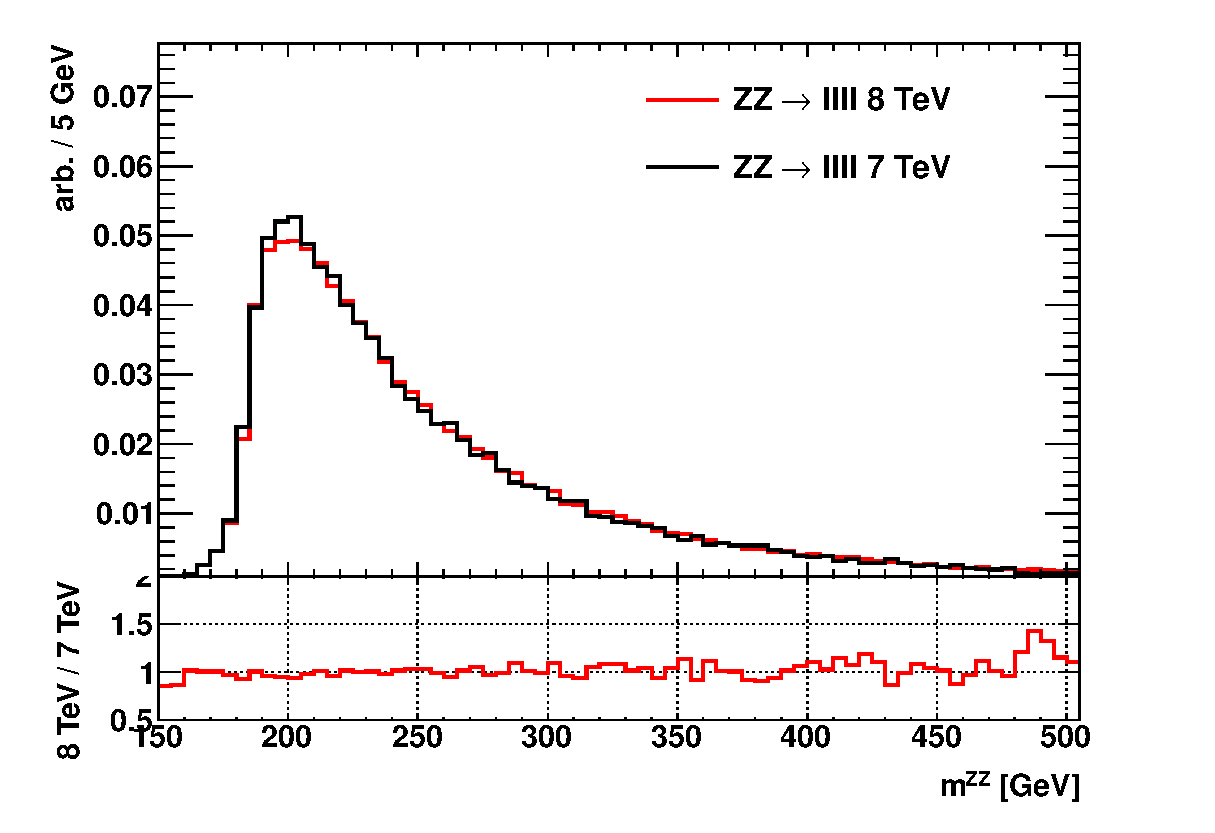
\includegraphics[width=0.47\textwidth]{Compare20112012/truth_ZZ_ZZ_m_lin}
    }
    \subfigure[]{
        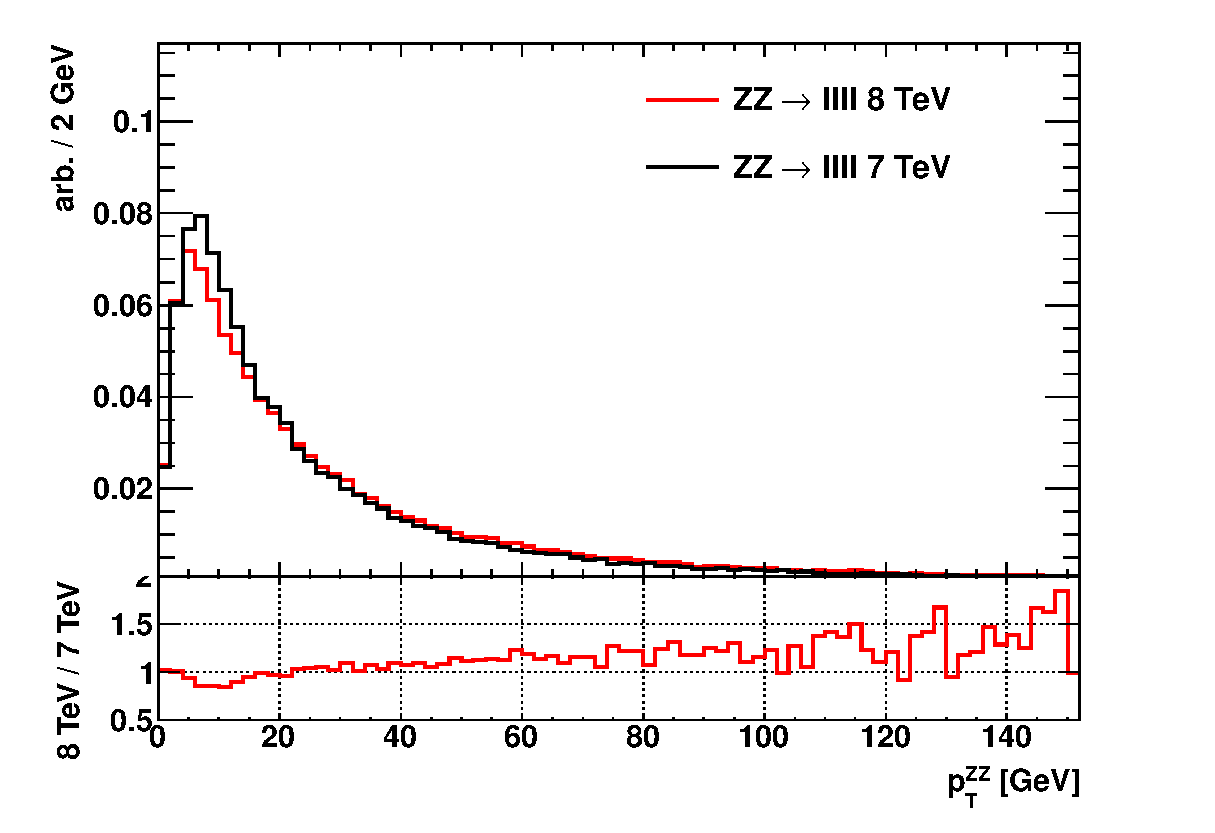
\includegraphics[width=0.47\textwidth]{Compare20112012/truth_ZZ_ZZ_pt_lin}
    }
        \vspace{-2mm}
    \subfigure[]{
        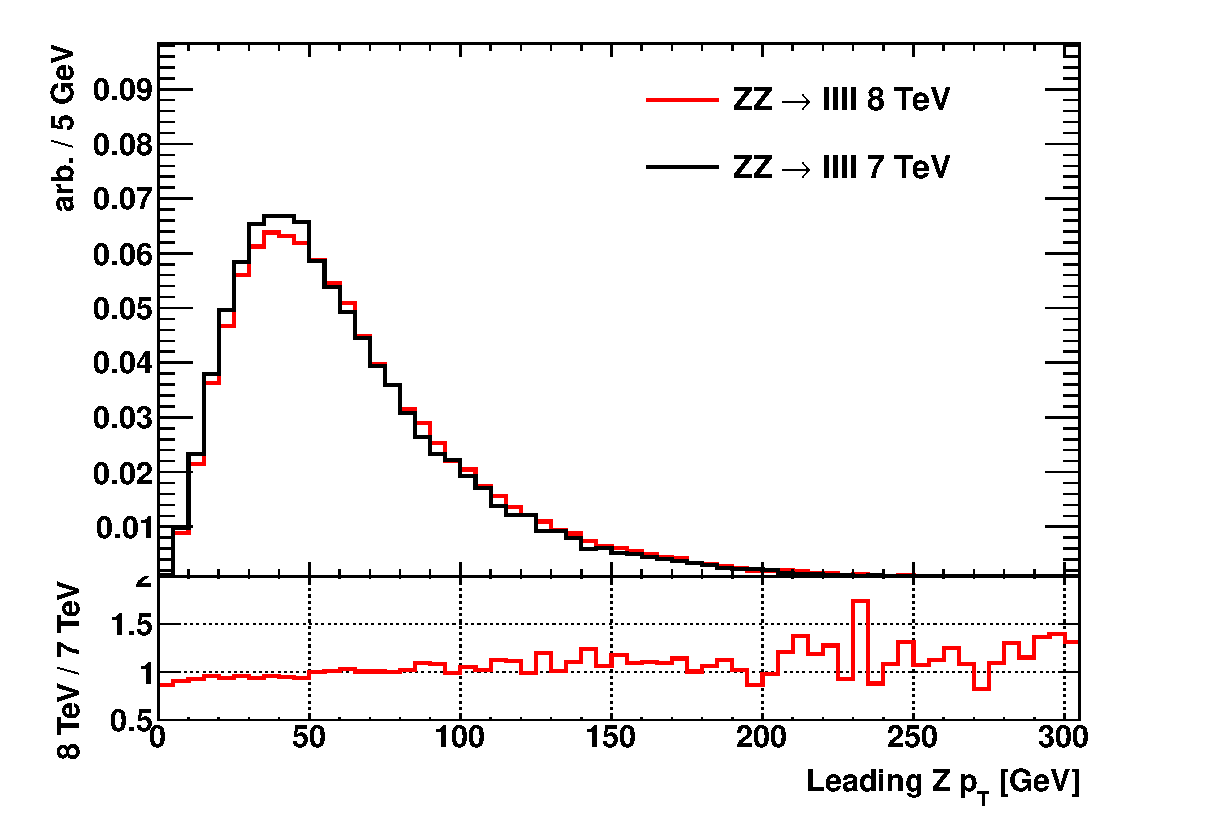
\includegraphics[width=0.47\textwidth]{Compare20112012/truth_ZZ_Z1_pt_lin}
    }
    \subfigure[]{
        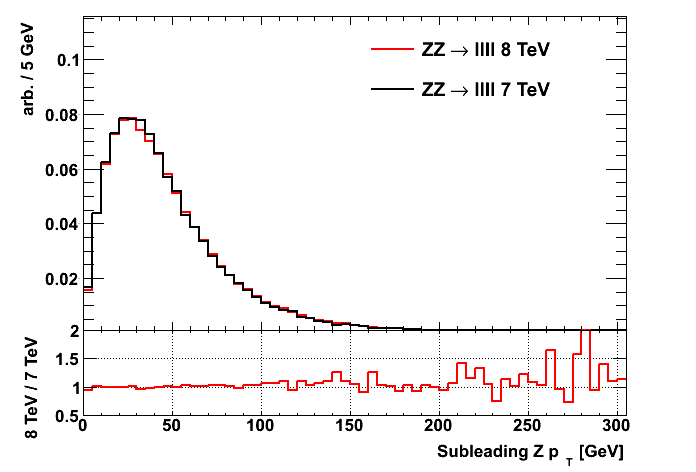
\includegraphics[width=0.47\textwidth]{Compare20112012/truth_ZZ_Z2_pt_lin}
    }
        \vspace{-2mm}
    \subfigure[]{
        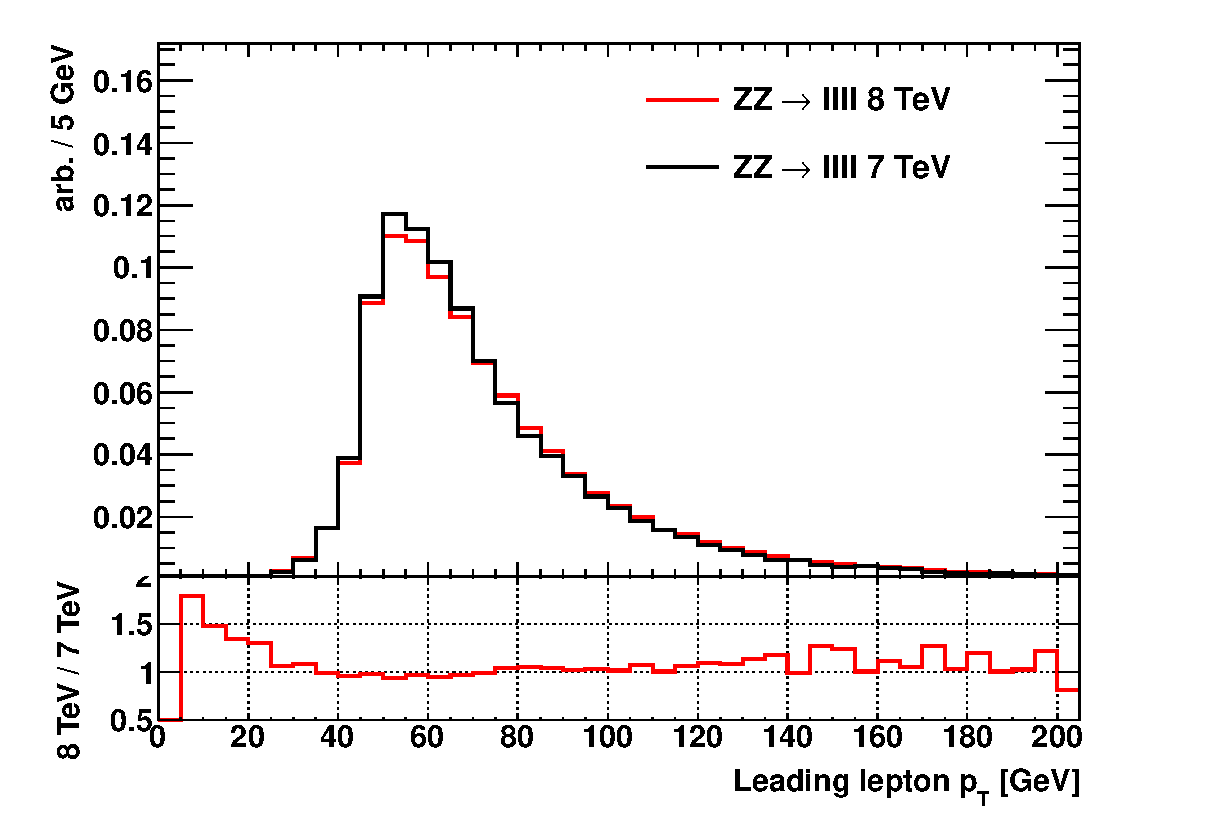
\includegraphics[width=0.47\textwidth]{Compare20112012/truth_ZZ_lep_1_pt_lin}
    }
    \subfigure[]{
        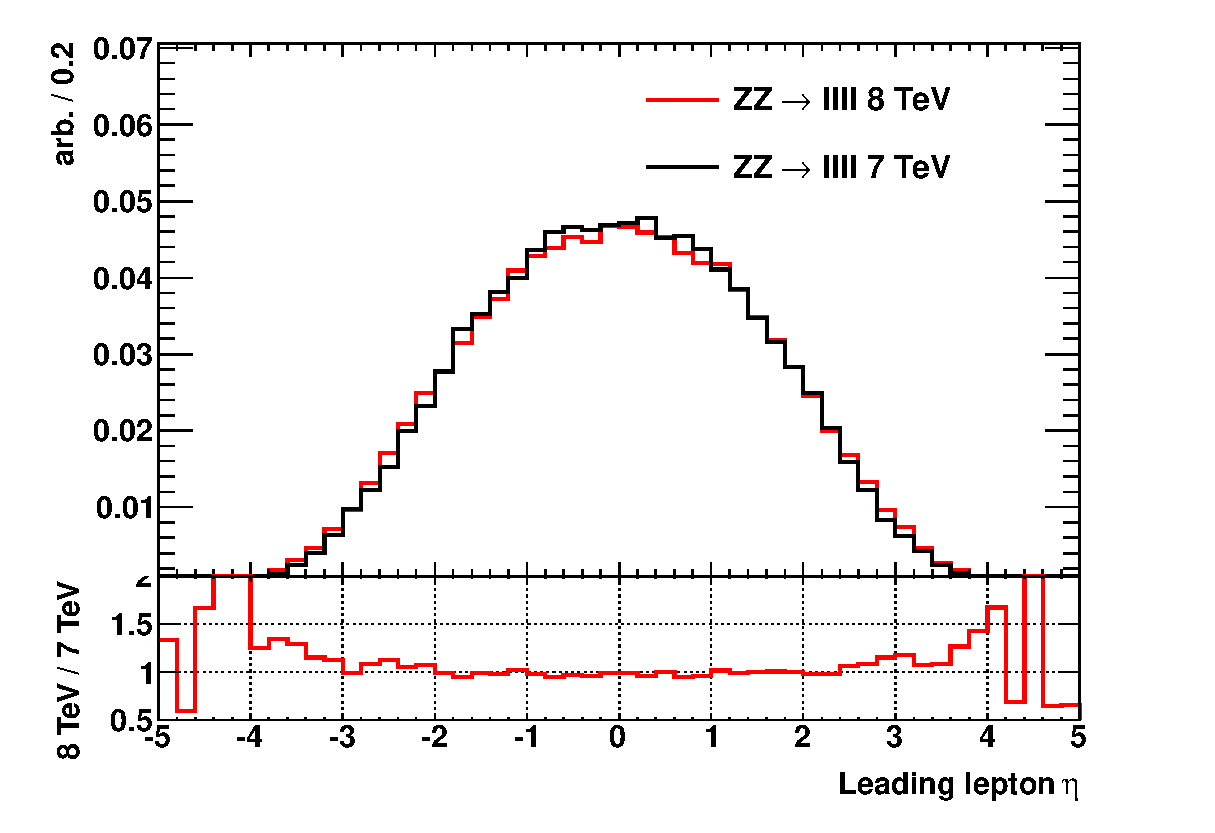
\includegraphics[width=0.47\textwidth]{Compare20112012/truth_ZZ_lep_1_eta_lin}
    }
        \vspace{-2mm}
    \subfigure[]{
        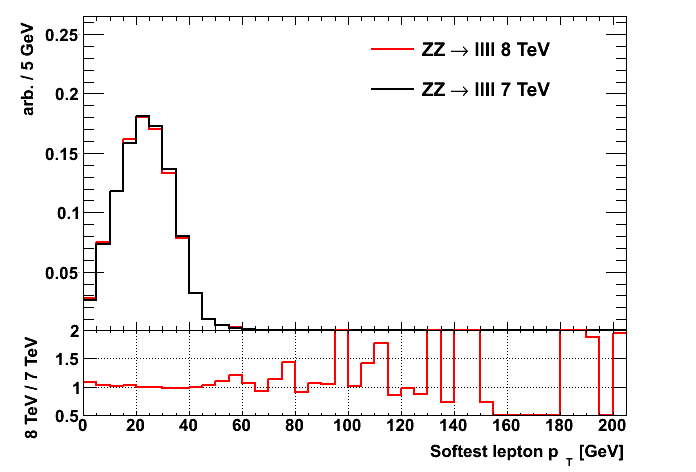
\includegraphics[width=0.47\textwidth]{Compare20112012/truth_ZZ_lep_4_pt_lin}
    }
    \subfigure[]{
        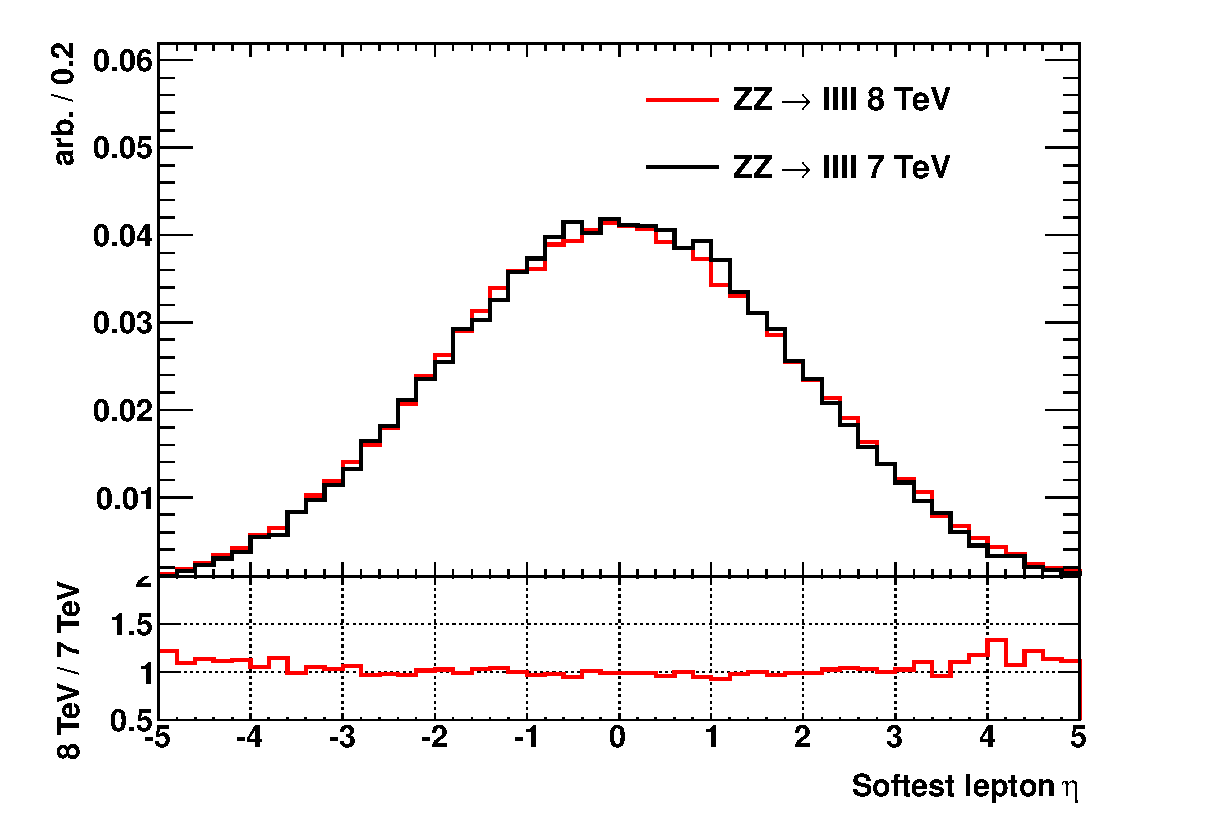
\includegraphics[width=0.47\textwidth]{Compare20112012/truth_ZZ_lep_4_eta_lin}
    }
        \vspace{-2mm}
    \caption{\small Comparison of generator level distributions, normalised to
    unit area, for \ZZllll\ for 7
    \tev\ and 8 \tev. Both \Z\ bosons are required to have \sstooosZ. Figures (a)
    and (b) show the mass and \pt\ of the \ZZ\ system,
    respectively. Figures (c) and (d) show the \pt\ of the
    leading and subleading \Z, respectively. Figure (e) shows the \pt\ of the highest \pt\ lepton in the event, and figure (f) shows its
   $\eta$. Similarly figures (g) and (h) show the \pt\ and $\eta$ of the lowest
   \pt\ lepton in the event.}
    \label{fig:gen-comp-7-8-ZZ}
\end{figure}

\begin{figure}
\centering
        \vspace{-5mm}
    \subfigure[]{
        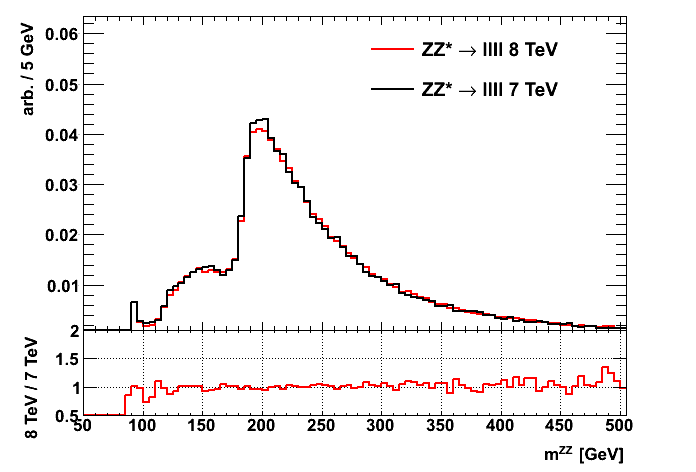
\includegraphics[width=0.47\textwidth]{Compare20112012/truth_ZZs_ZZ_m_lin}
    }
    \subfigure[]{
        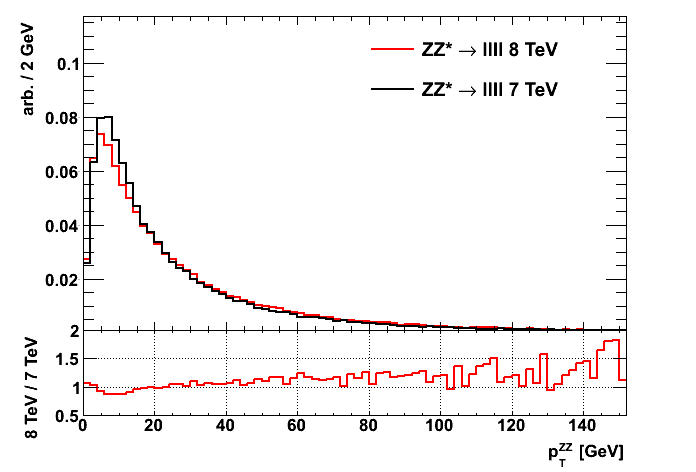
\includegraphics[width=0.47\textwidth]{Compare20112012/truth_ZZs_ZZ_pt_lin}
    }
        \vspace{-2mm}
    \subfigure[]{
        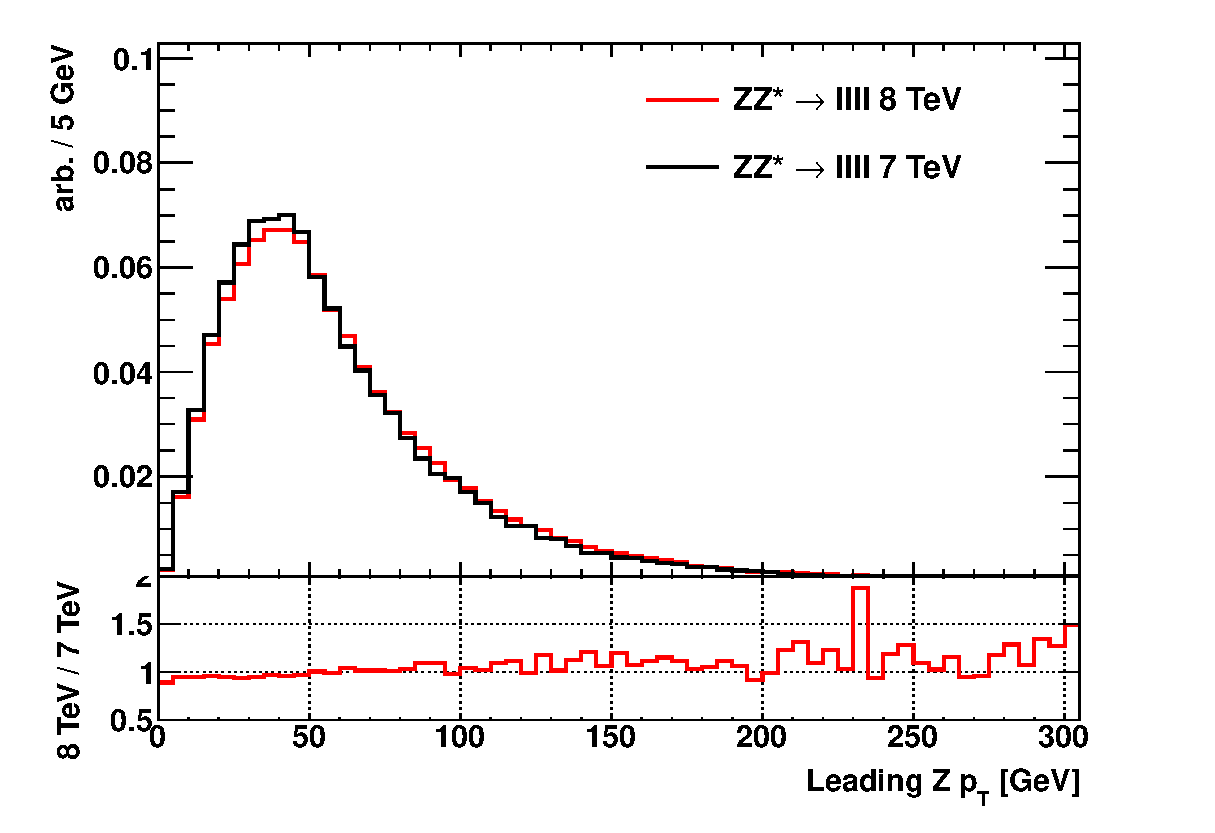
\includegraphics[width=0.47\textwidth]{Compare20112012/truth_ZZs_Z1_pt_lin}
    }
    \subfigure[]{
        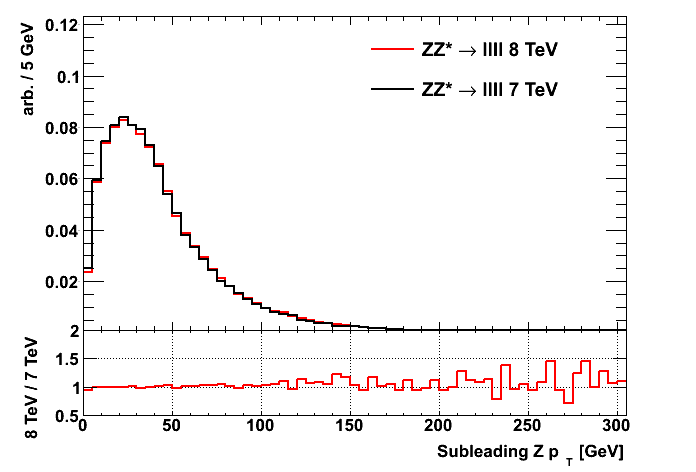
\includegraphics[width=0.47\textwidth]{Compare20112012/truth_ZZs_Z2_pt_lin}
    }
        \vspace{-2mm}
    \subfigure[]{
        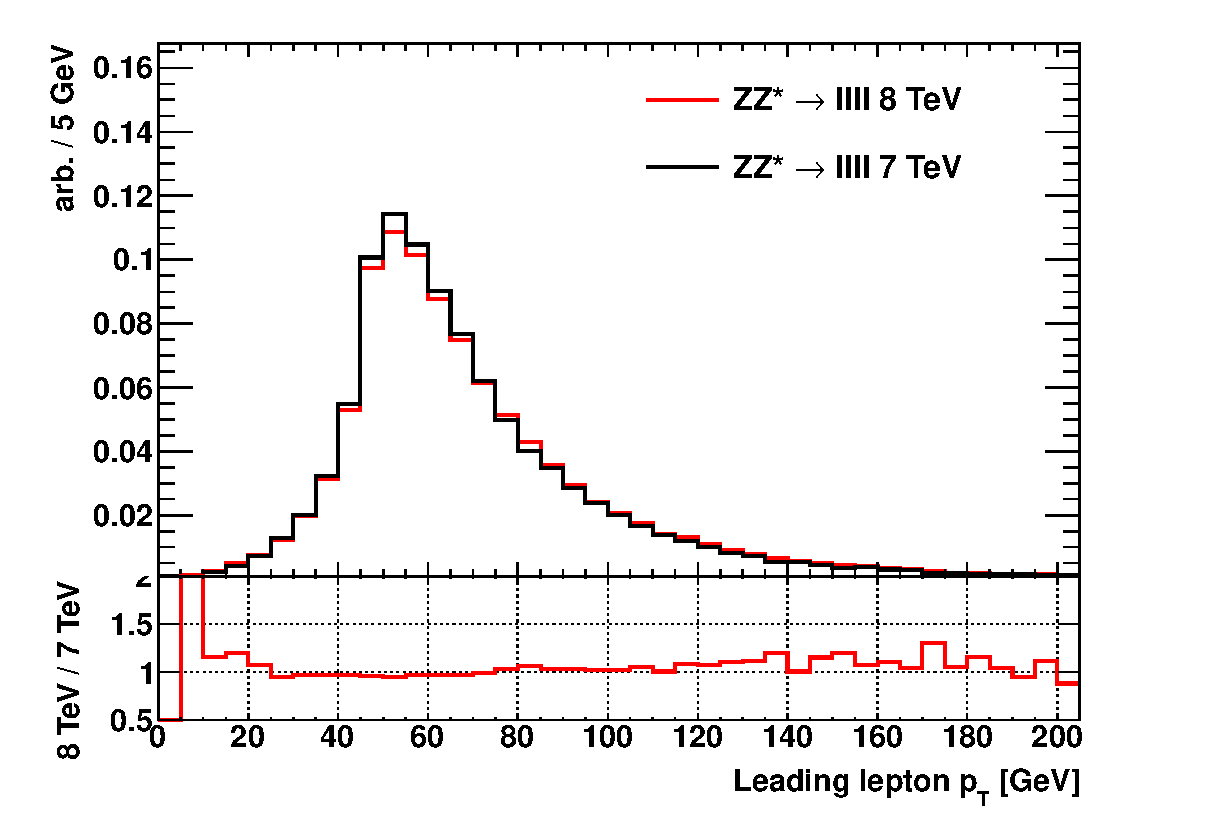
\includegraphics[width=0.47\textwidth]{Compare20112012/truth_ZZs_lep_1_pt_lin}
    }
    \subfigure[]{
        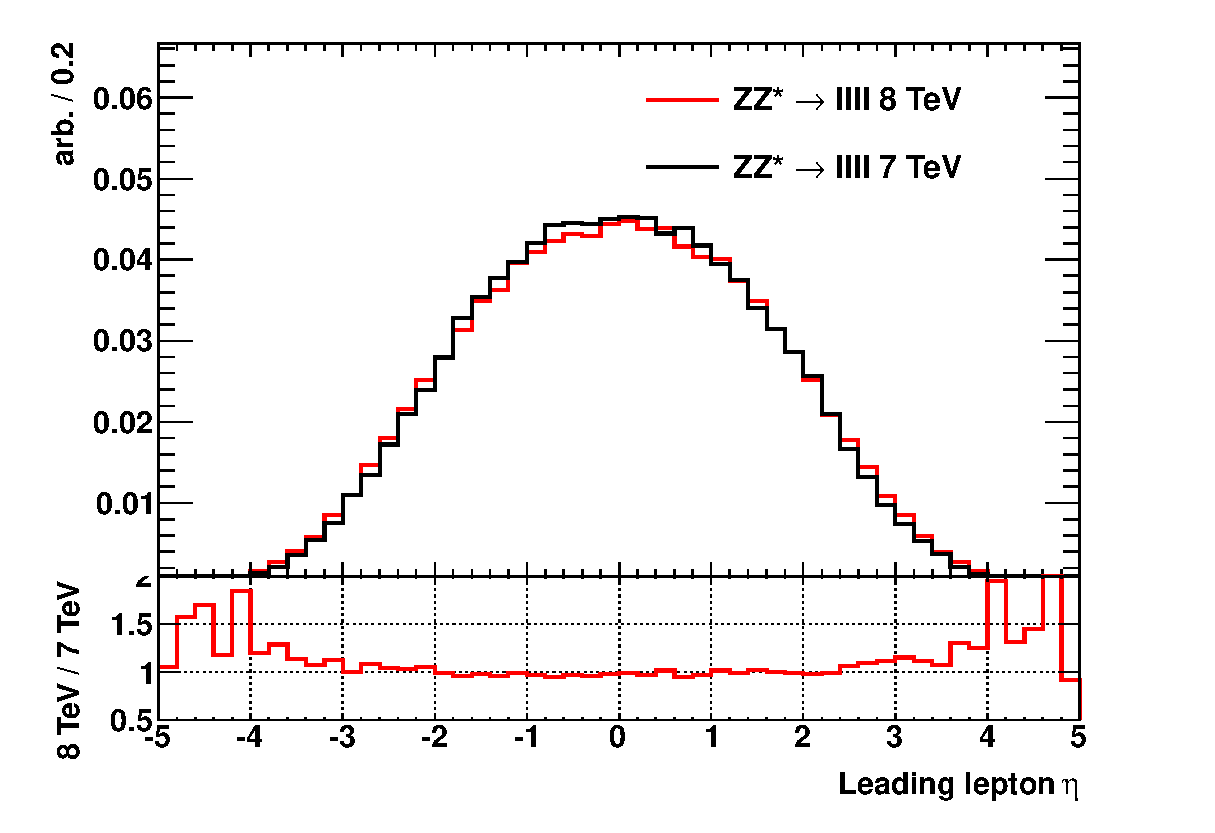
\includegraphics[width=0.47\textwidth]{Compare20112012/truth_ZZs_lep_1_eta_lin}
    }
        \vspace{-2mm}
    \subfigure[]{
        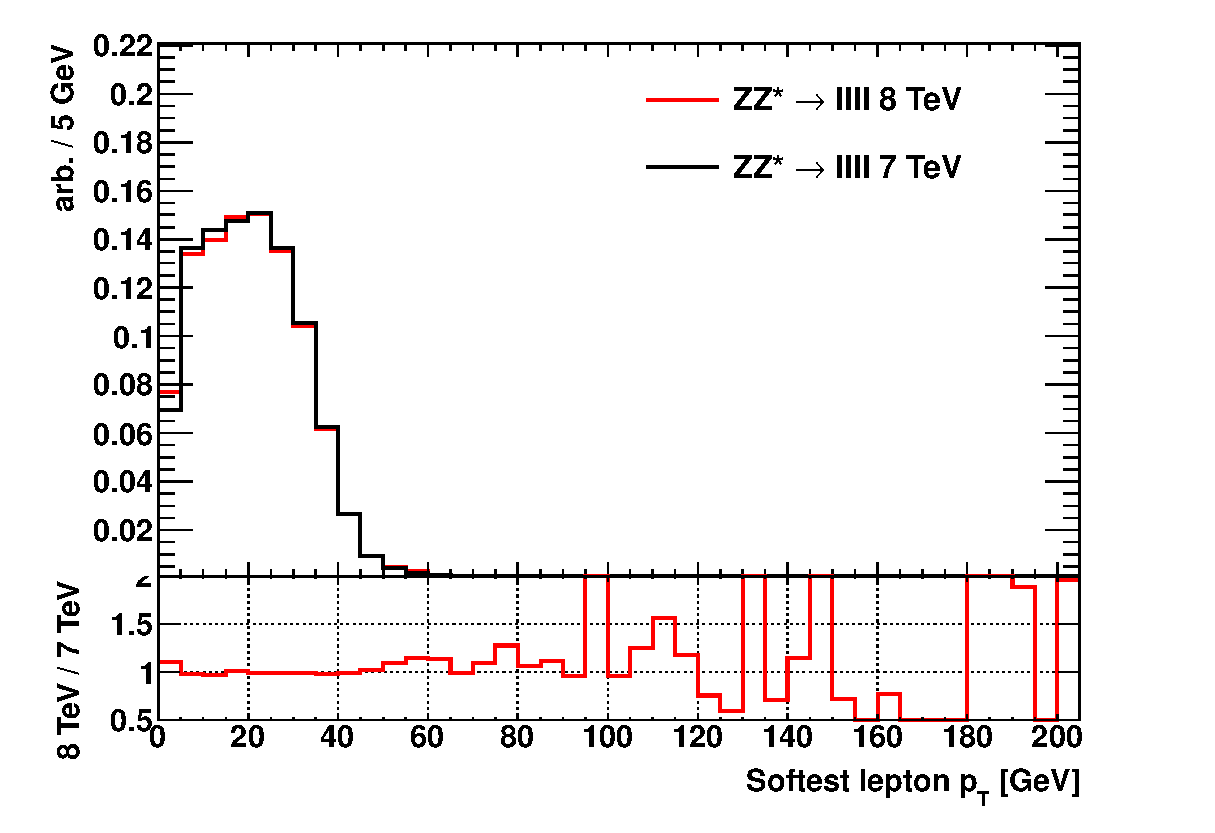
\includegraphics[width=0.47\textwidth]{Compare20112012/truth_ZZs_lep_4_pt_lin}
    }
    \subfigure[]{
        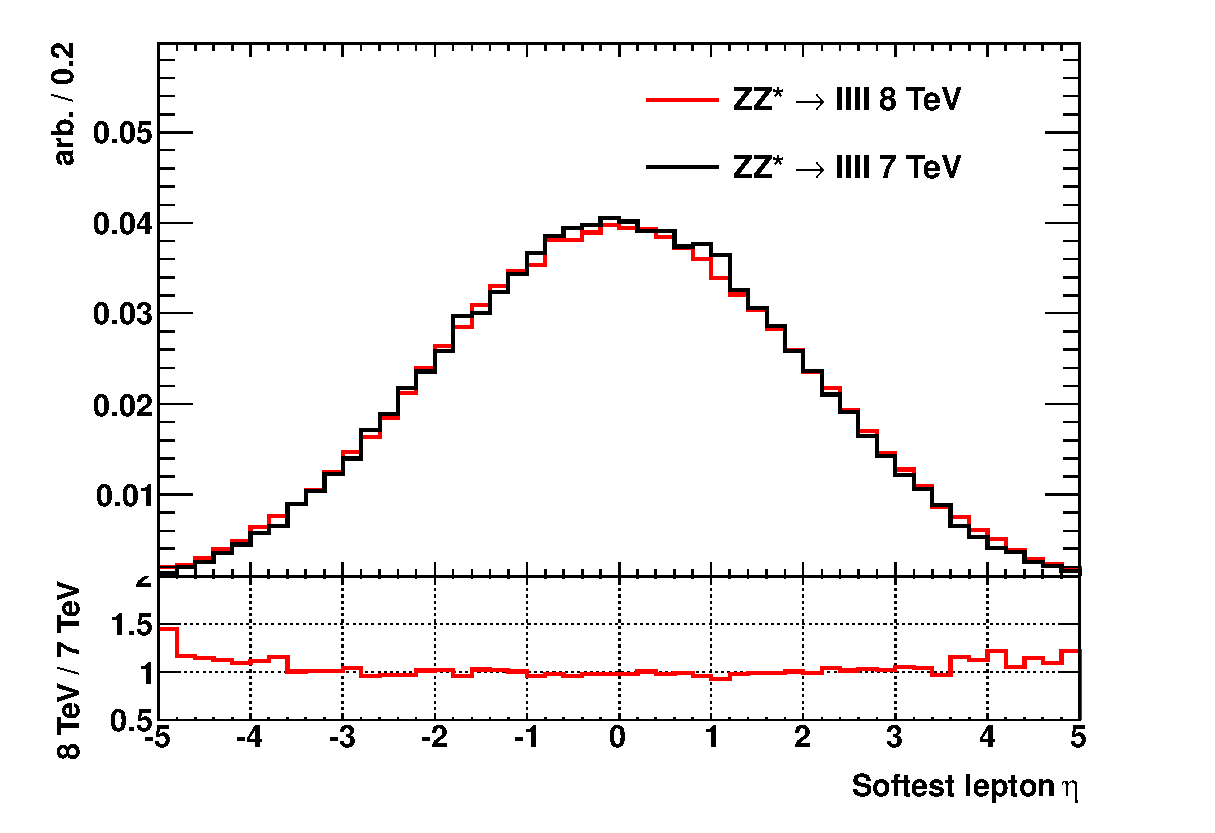
\includegraphics[width=0.47\textwidth]{Compare20112012/truth_ZZs_lep_4_eta_lin}
    }
        \vspace{-2mm}
    \caption{\small Comparison of generator level distributions, normalised to
    unit area, for \ZZsllll\ for 7
    \tev\ and 8 \tev. One \Z\ is required to have \sstooosZ\ and the other
    \mZgtt. Figures (a)
    and (b) show the mass and \pt\ of the \ZZ\ system,
    respectively. Figures (c) and (d) show the \pt\ of the
    leading and subleading \Z, respectively. Figure (e) shows the \pt\ of the highest \pt\ lepton in the event, and figure (f) shows its
   $\eta$. Similarly figures (g) and (h) show the \pt\ and $\eta$ of the lowest
   \pt\ lepton in the event.}
    \label{fig:gen-comp-7-8-ZZs}
\end{figure}

\subsection{Comparison of \ggZZ\ and \qqZZ}

~\fig{gen-comp-gg-qq-ZZ} shows a comparison of kinematic distributions in \ggZZ\ 
(simulated using \ggtwoZZ) and \qqZZ events (simulated using \powhegbox), 
requiring that both \Z\ bosons have \sstooos. ~\fig{gen-comp-gg-qq-ZZs} shows 
the same distributions after relaxing the requirement on the \Z\ furthest from 
the pole to $m_{Z}>20$ \gev. The \mZZ\ distribution is similar in both 
processes, however the \ptZZ\ distribution is much harder in the case of \ggZZ.  
This can be attributed to increased initial state radiation in the gluon-gluon 
fusion process. As a consequence of this, the leading \Z\ \pt\ distribution is 
slightly harder in the \ggZZ\ process, whilst the subleading \Z\ \pt\ is 
slightly softer. The leptons produced in \ggZZ\ decays are much more central, 
and have slightly higher \pt\ on average than in \qqZZ\ decays.

\begin{figure}
\centering
        \vspace{-5mm}
    \subfigure[]{
        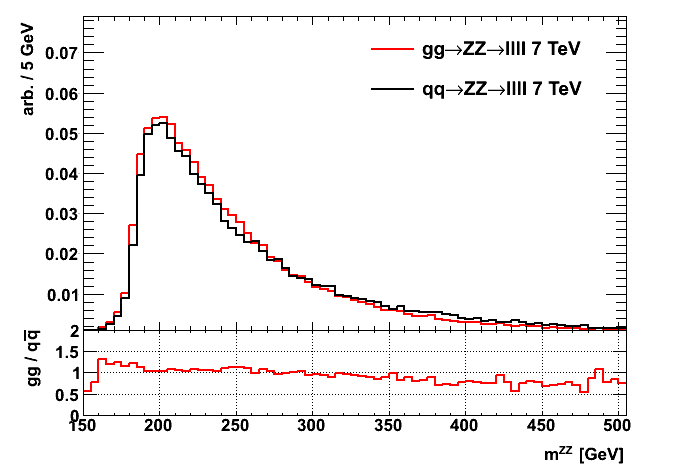
\includegraphics[width=0.47\textwidth]{Compareggqq7TeV/truth_ZZ_ZZ_m_lin}
    }
    \subfigure[]{
        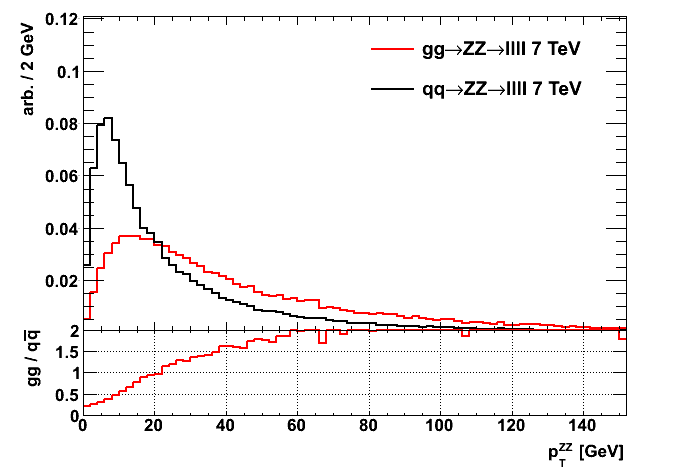
\includegraphics[width=0.47\textwidth]{Compareggqq7TeV/truth_ZZ_ZZ_pt_lin}
    }
        \vspace{-2mm}
    \subfigure[]{
        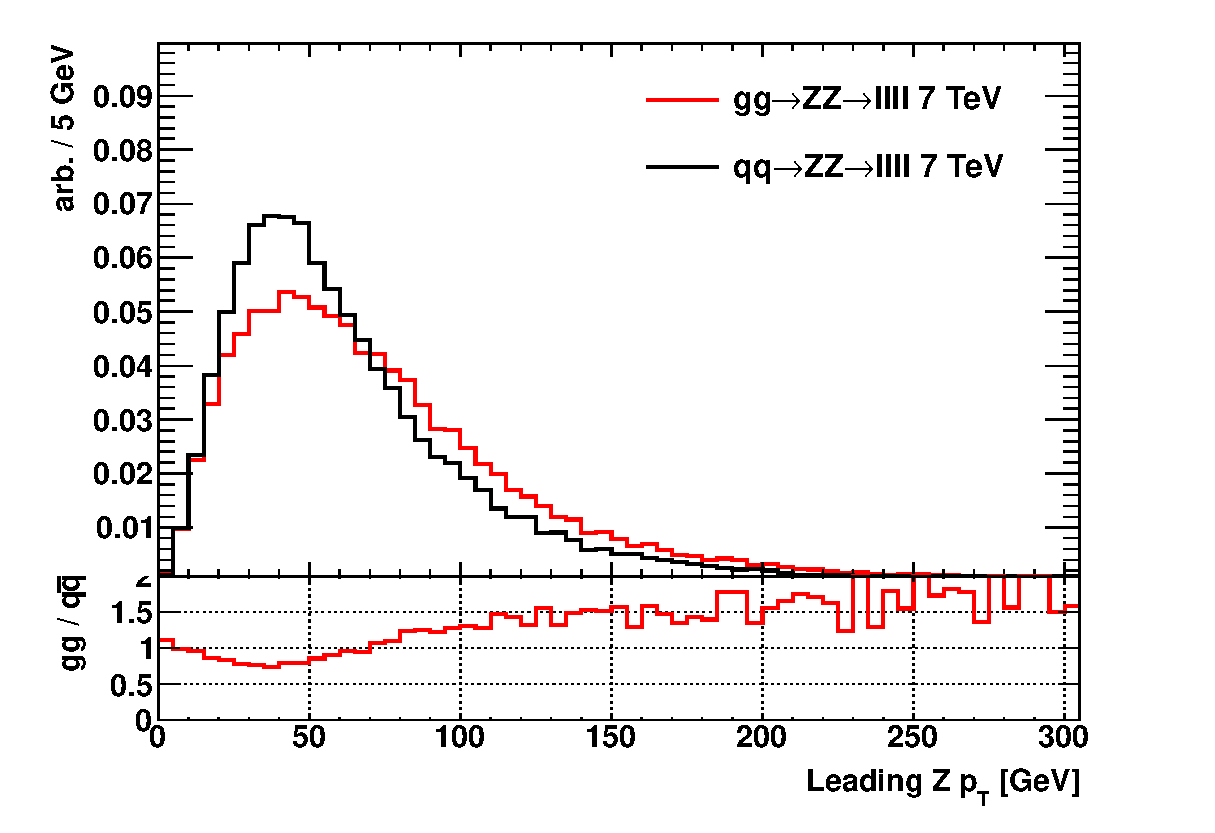
\includegraphics[width=0.47\textwidth]{Compareggqq7TeV/truth_ZZ_Z1_pt_lin}
    }
    \subfigure[]{
        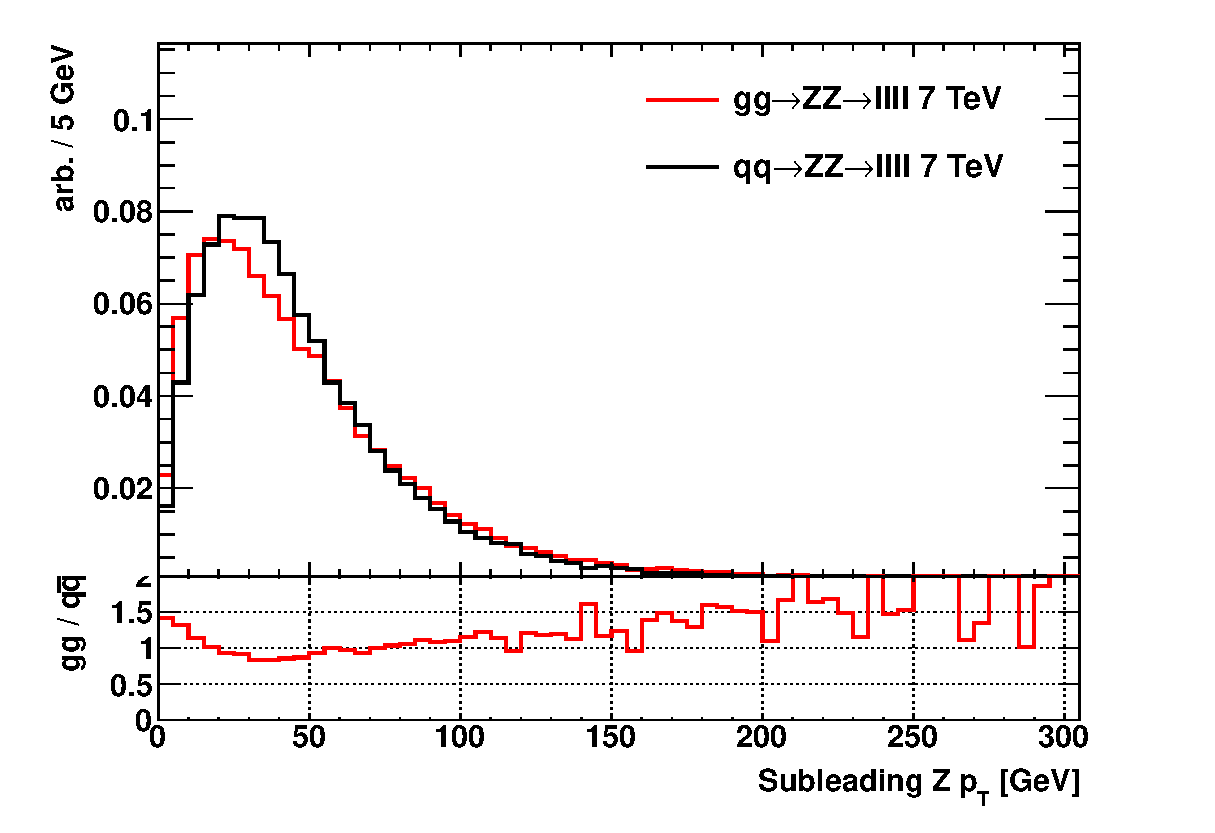
\includegraphics[width=0.47\textwidth]{Compareggqq7TeV/truth_ZZ_Z2_pt_lin}
    }
        \vspace{-2mm}
    \subfigure[]{
        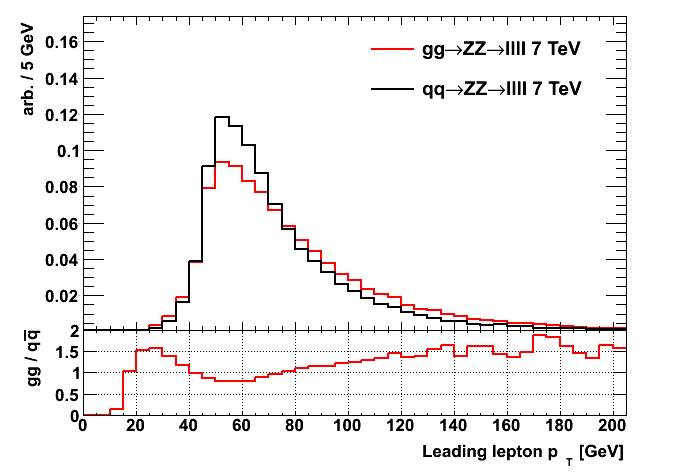
\includegraphics[width=0.47\textwidth]{Compareggqq7TeV/truth_ZZ_lep_1_pt_lin}
    }
    \subfigure[]{
        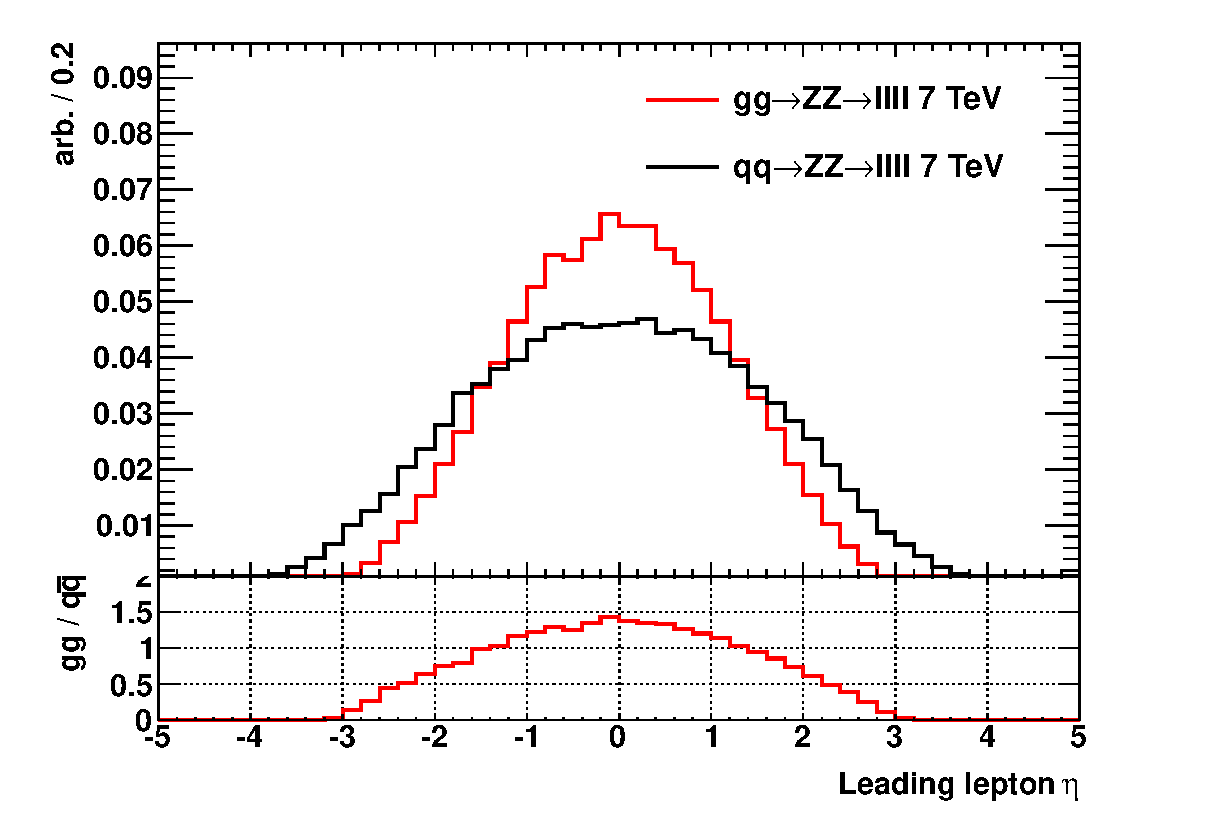
\includegraphics[width=0.47\textwidth]{Compareggqq7TeV/truth_ZZ_lep_1_eta_lin}
    }
        \vspace{-2mm}
    \subfigure[]{
        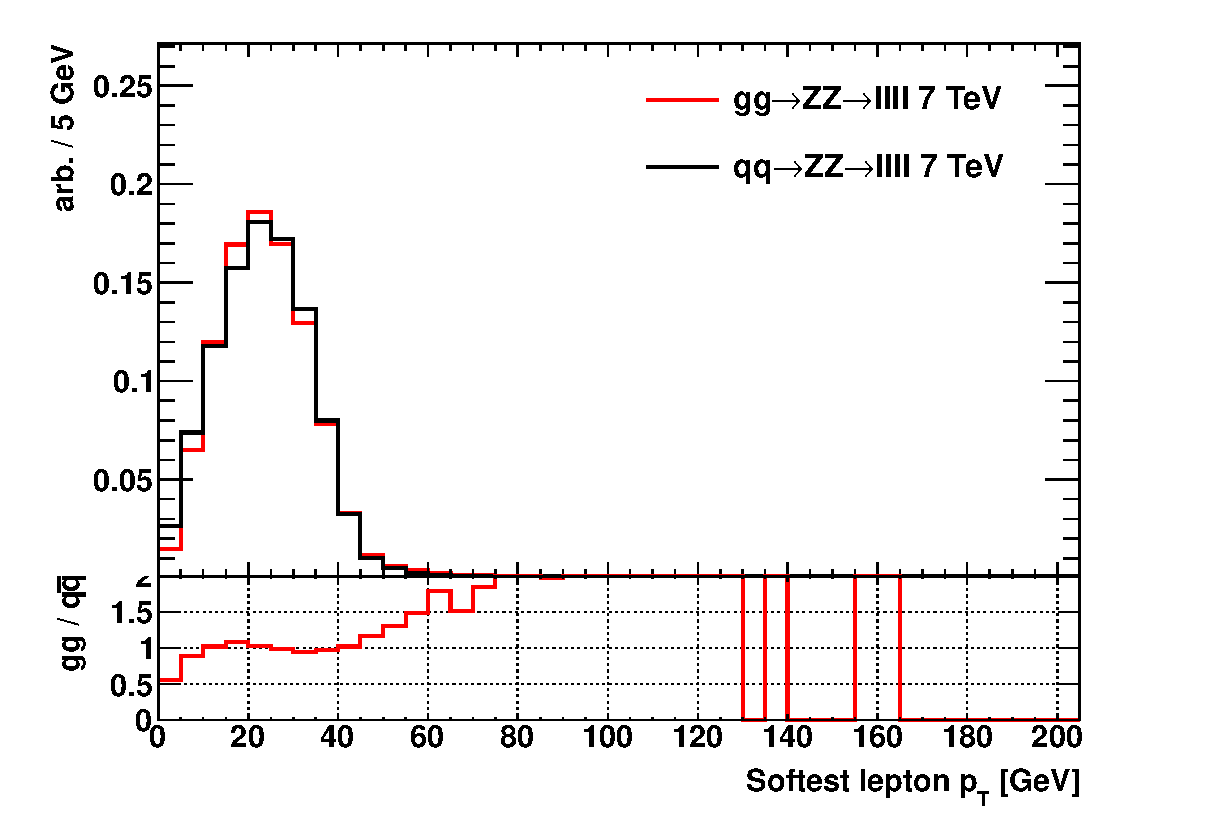
\includegraphics[width=0.47\textwidth]{Compareggqq7TeV/truth_ZZ_lep_4_pt_lin}
    }
    \subfigure[]{
        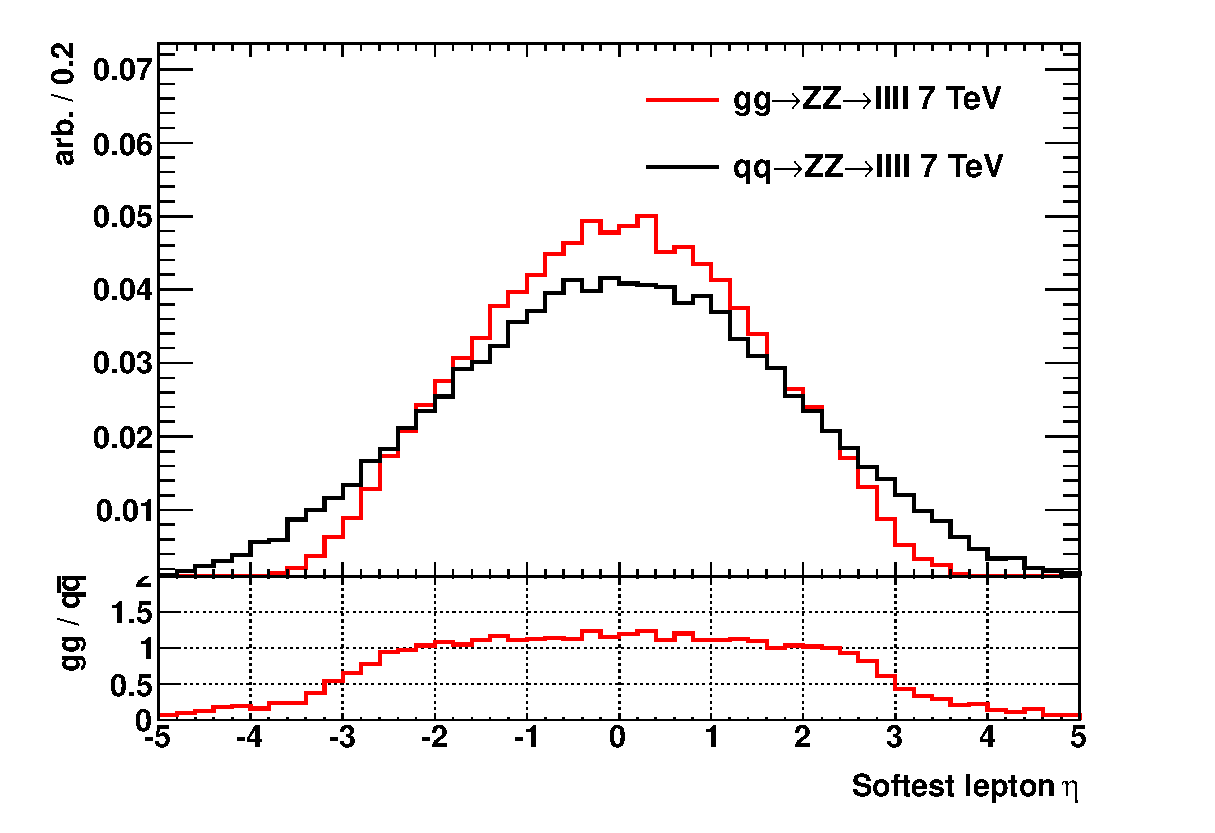
\includegraphics[width=0.47\textwidth]{Compareggqq7TeV/truth_ZZ_lep_4_eta_lin}
    }
        \vspace{-2mm}
    \caption{\small Comparison of generator level distributions, normalised to
    unit area, for \ZZllll\ proceeding via $qq$ and $gg$ interactions. Both \Z\
    bosons are required to have \sstooosZ. Figures (a)
    and (b) show the mass and \pt\ of the \ZZ\ system,
    respectively. Figures (c) and (d) show the \pt\ of the
    leading and subleading \Z, respectively. Figure (e) shows the \pt\ of the highest \pt\ lepton in the event, and figure (f) shows its
   $\eta$. Similarly figures (g) and (h) show the \pt\ and $\eta$ of the lowest
   \pt\ lepton in the event.}
    \label{fig:gen-comp-gg-qq-ZZ}
\end{figure}

\begin{figure}
\centering
        \vspace{-5mm}
    \subfigure[]{
        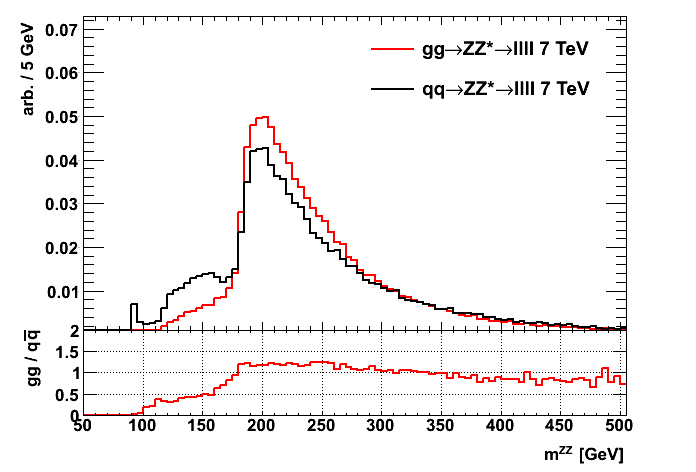
\includegraphics[width=0.47\textwidth]{Compareggqq7TeV/truth_ZZs_ZZ_m_lin}
    }
    \subfigure[]{
        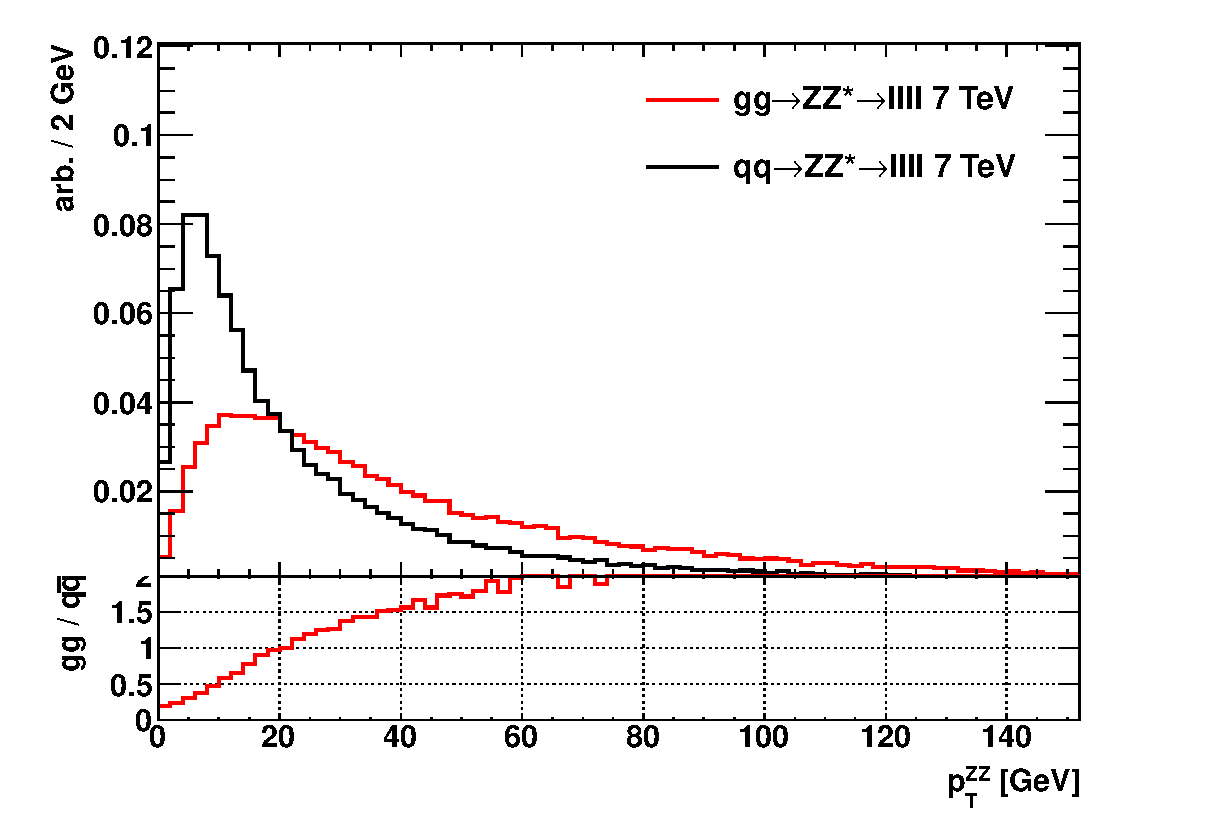
\includegraphics[width=0.47\textwidth]{Compareggqq7TeV/truth_ZZs_ZZ_pt_lin}
    }
        \vspace{-2mm}
    \subfigure[]{
        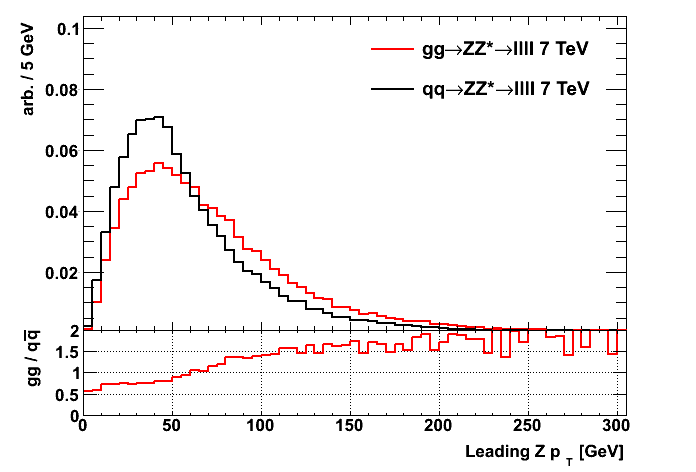
\includegraphics[width=0.47\textwidth]{Compareggqq7TeV/truth_ZZs_Z1_pt_lin}
    }
    \subfigure[]{
        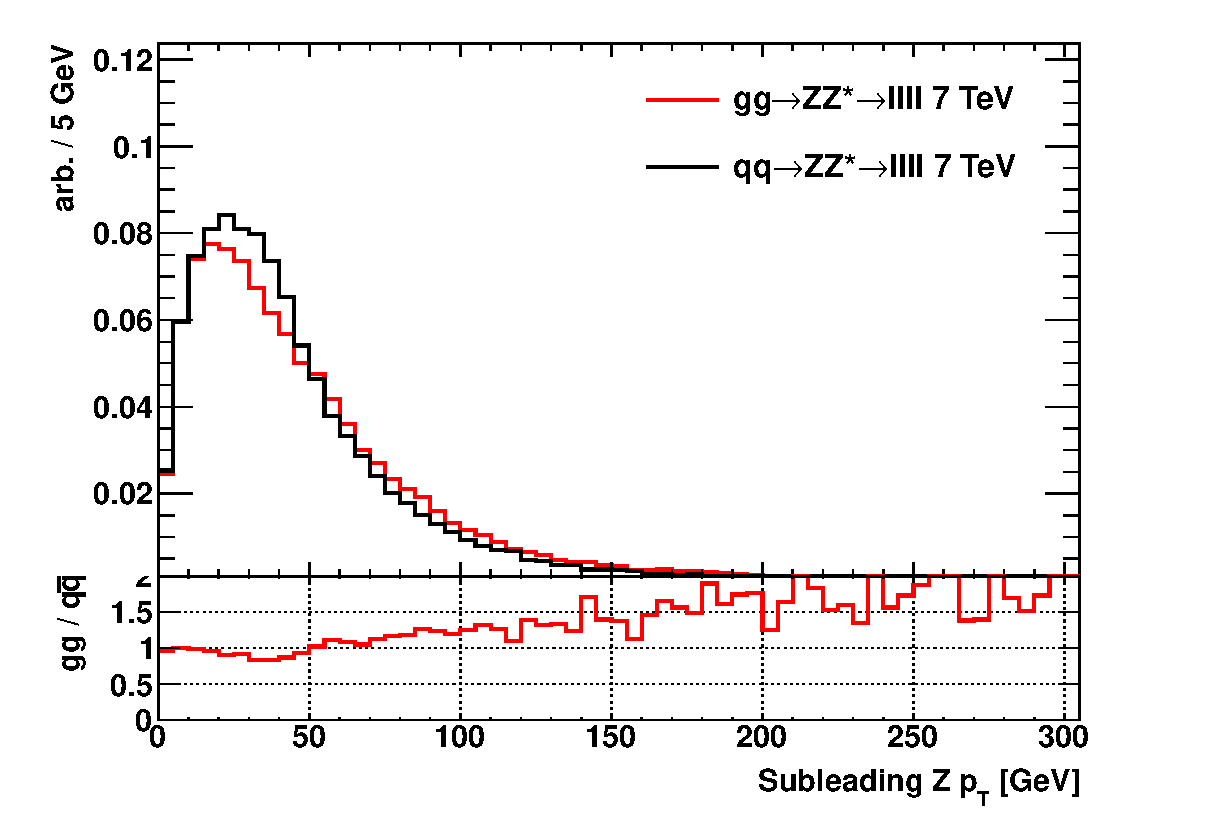
\includegraphics[width=0.47\textwidth]{Compareggqq7TeV/truth_ZZs_Z2_pt_lin}
    }
        \vspace{-2mm}
    \subfigure[]{
        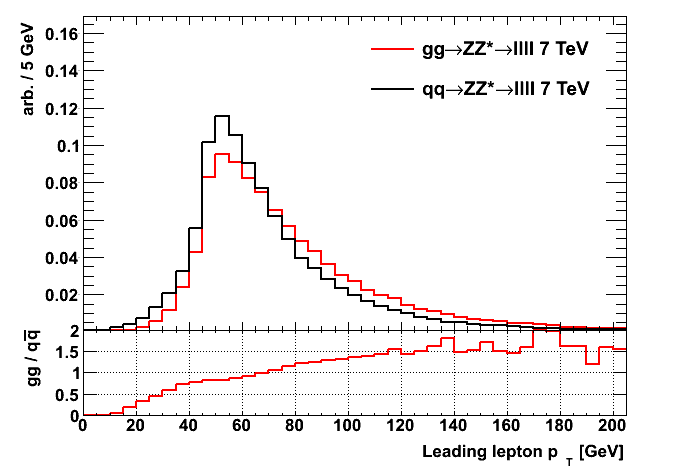
\includegraphics[width=0.47\textwidth]{Compareggqq7TeV/truth_ZZs_lep_1_pt_lin}
    }
    \subfigure[]{
        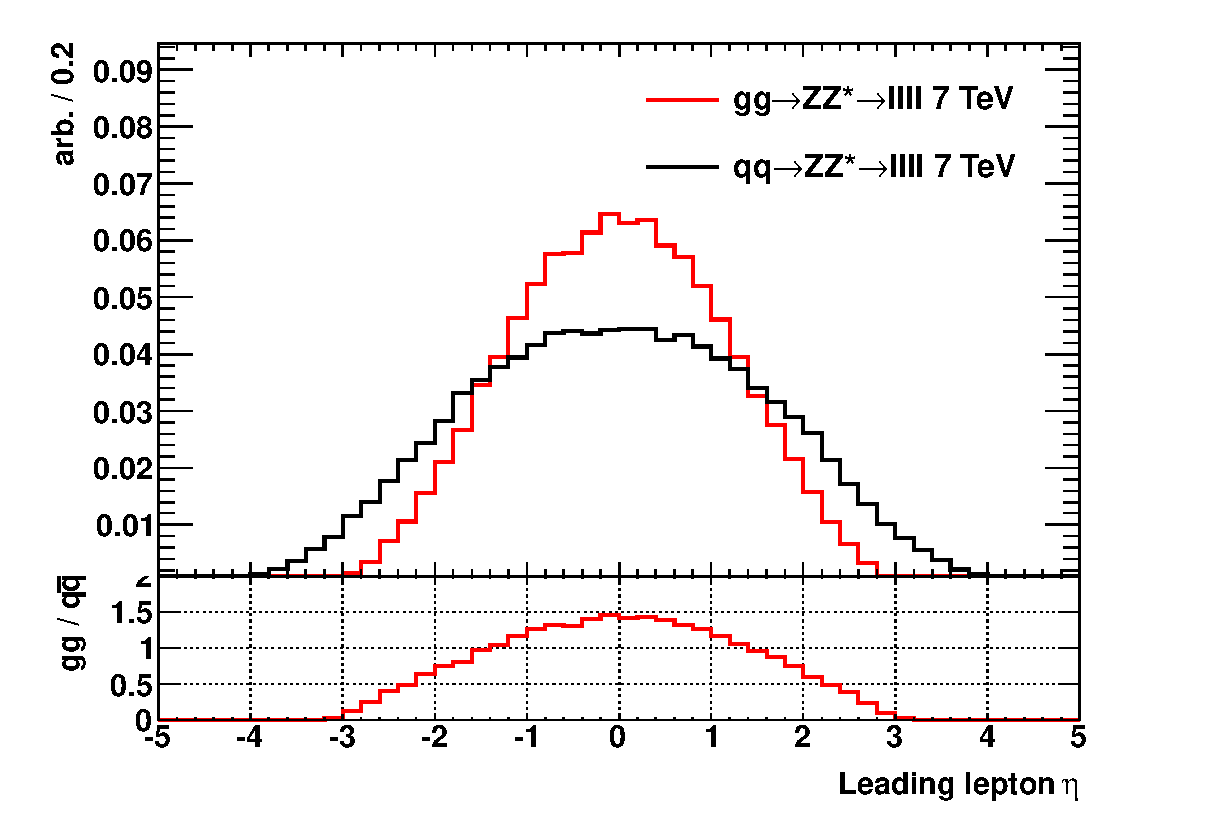
\includegraphics[width=0.47\textwidth]{Compareggqq7TeV/truth_ZZs_lep_1_eta_lin}
    }
        \vspace{-2mm}
    \subfigure[]{
        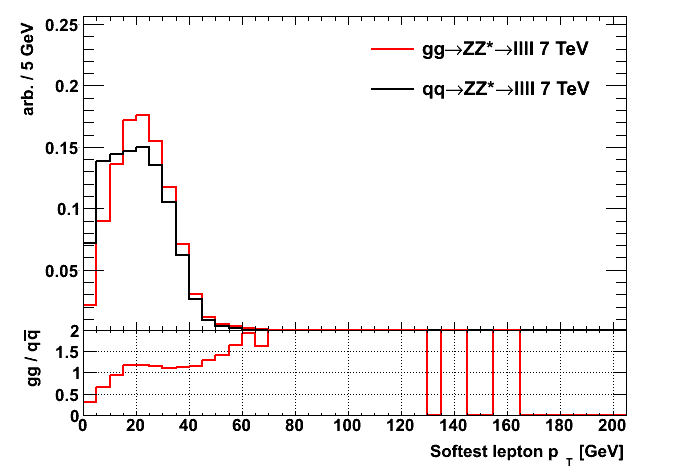
\includegraphics[width=0.47\textwidth]{Compareggqq7TeV/truth_ZZs_lep_4_pt_lin}
    }
    \subfigure[]{
        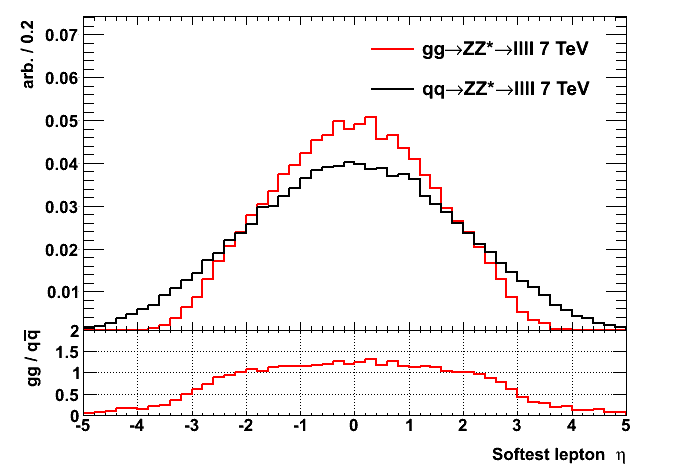
\includegraphics[width=0.47\textwidth]{Compareggqq7TeV/truth_ZZs_lep_4_eta_lin}
    }
        \vspace{-2mm}
    \caption{\small Comparison of generator level distributions, normalised to
    unit area, for \ZZsllll\ proceeding via $qq$ and $gg$ interactions. One \Z\ is required to have \sstooos\ and the other
    $m_{Z}>20$ \gev. Figures (a)
    and (b) show the mass and \pt\ of the \ZZ\ system,
    respectively. Figures (c) and (d) show the \pt\ of the
    leading and subleading \Z, respectively. Figure (e) shows the \pt\ of the highest \pt\ lepton in the event, and figure (f) shows its
   $\eta$. Similarly figures (g) and (h) show the \pt\ and $\eta$ of the lowest
   \pt\ lepton in the event.}
    \label{fig:gen-comp-gg-qq-ZZs}
\end{figure}


\subsection{Generator Comparisons for \ZZllll}

\begin{figure}
\centering
        \vspace{-5mm}
    \subfigure[]{
        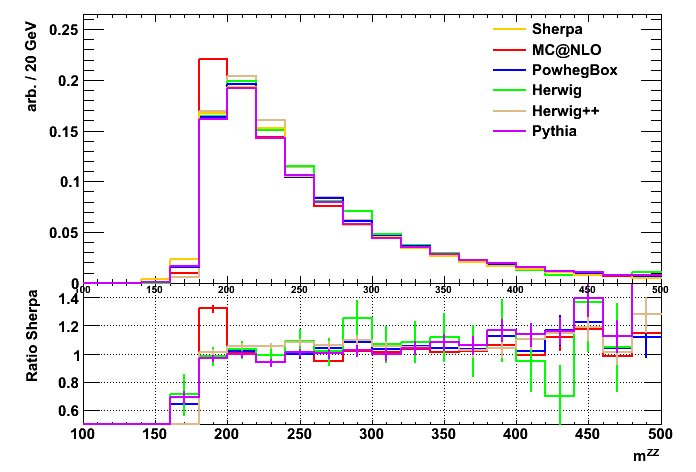
\includegraphics[width=0.47\textwidth]{GeneratorComparison/fidZZ_ZZ_m_2e2mu_wRatio_linear}
    }
    \subfigure[]{
        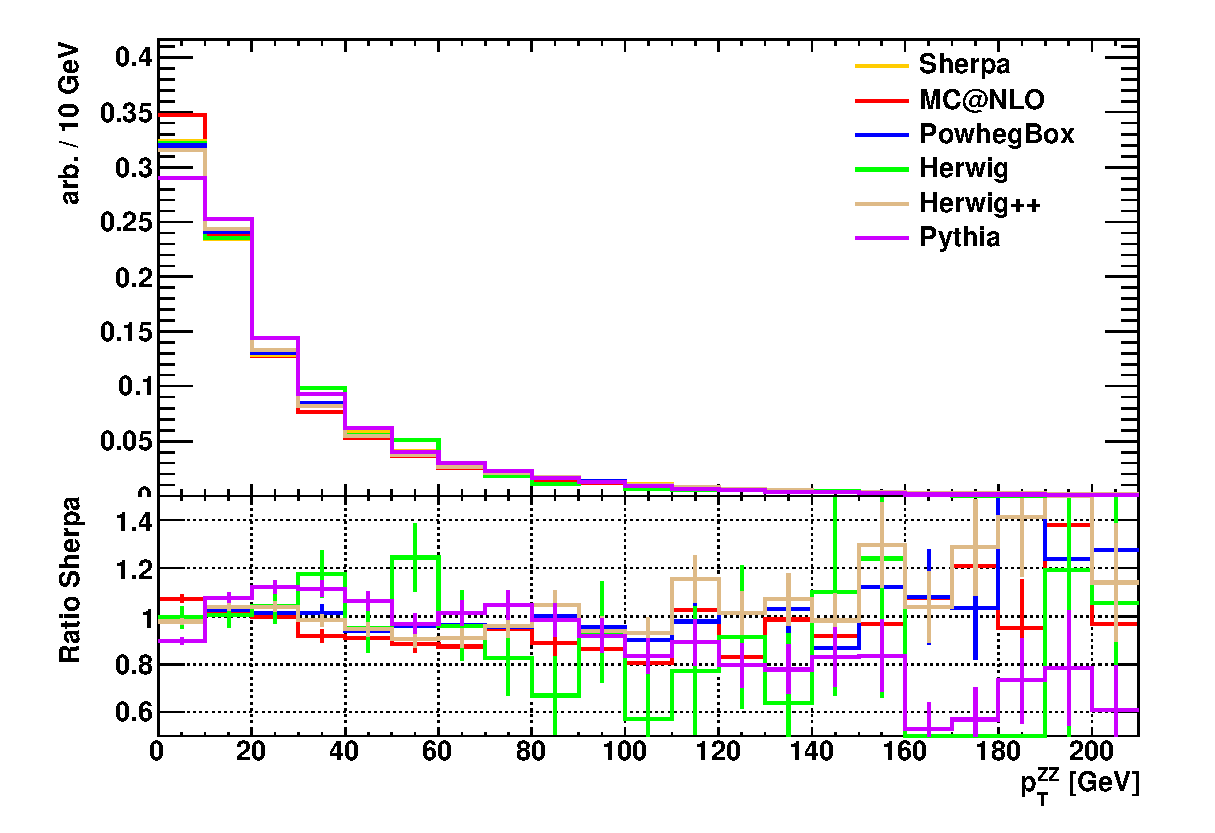
\includegraphics[width=0.47\textwidth]{GeneratorComparison/fidZZ_ZZ_pt_2e2mu_wRatio_linear}
    }
        \vspace{-2mm}
    \subfigure[]{
        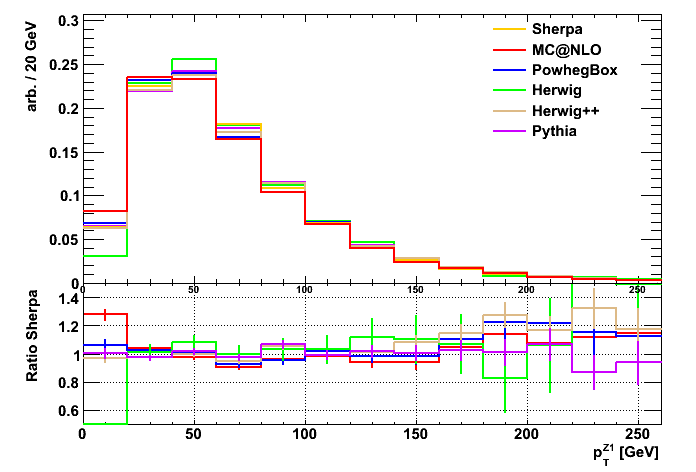
\includegraphics[width=0.47\textwidth]{GeneratorComparison/fidZZ_Z1_pt_2e2mu_wRatio_linear}
    }
    \subfigure[]{
        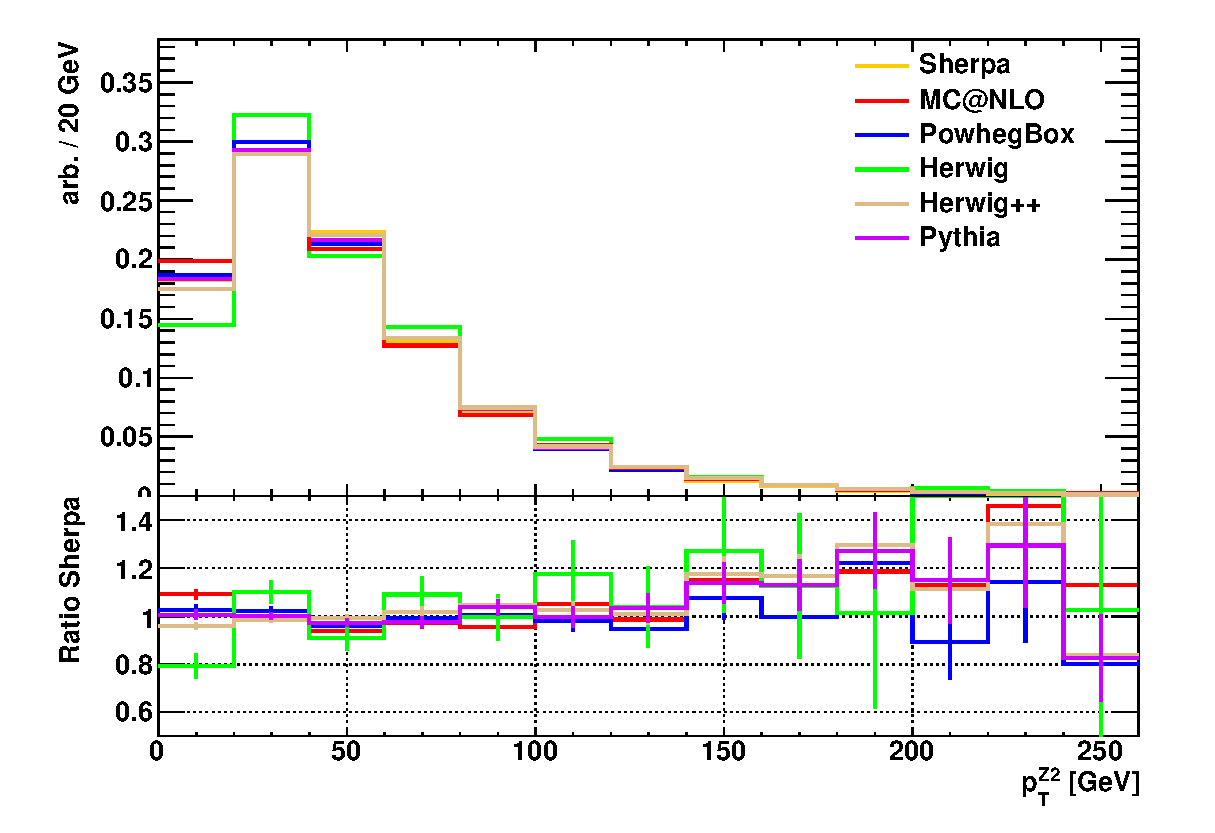
\includegraphics[width=0.47\textwidth]{GeneratorComparison/fidZZ_Z2_pt_2e2mu_wRatio_linear}
    }
        \vspace{-2mm}
    \subfigure[]{
        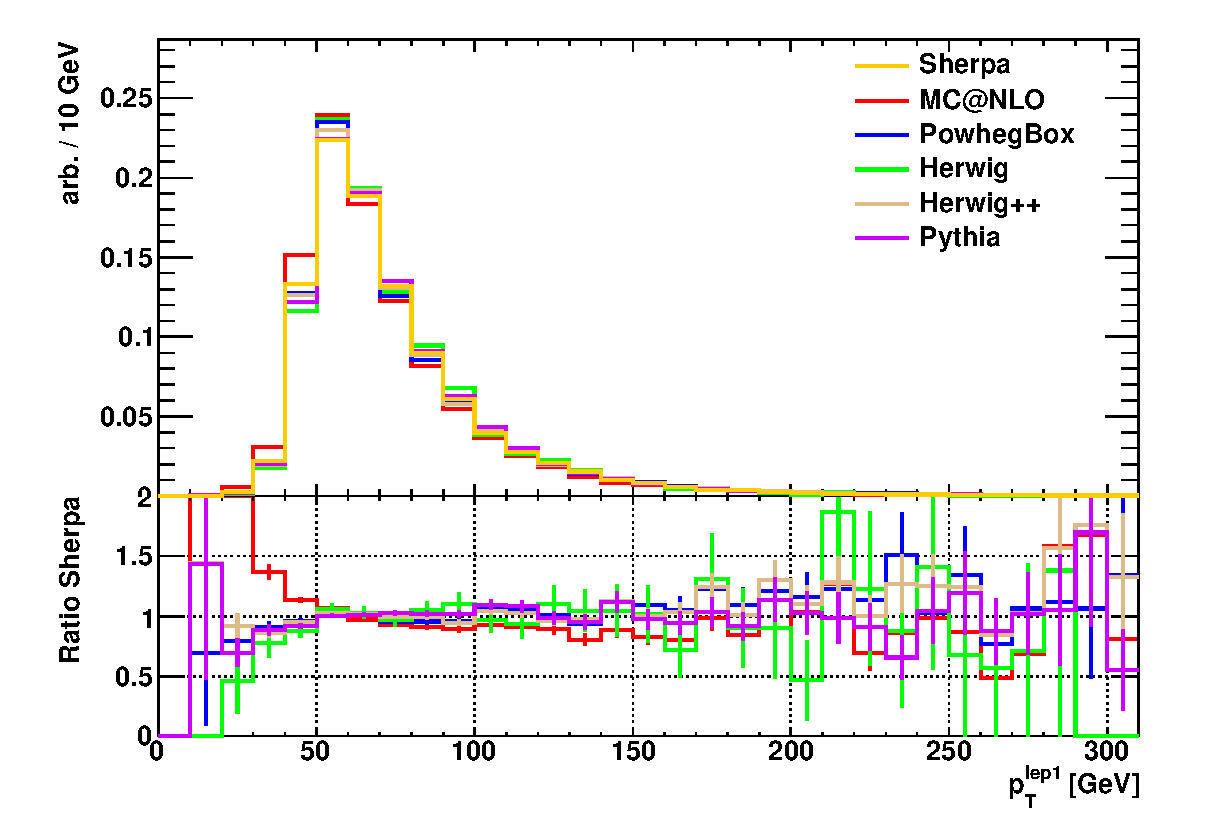
\includegraphics[width=0.47\textwidth]{GeneratorComparison/ZZ_lep_1_pt_2e2mu_wRatio_linear}
    }
    \subfigure[]{
        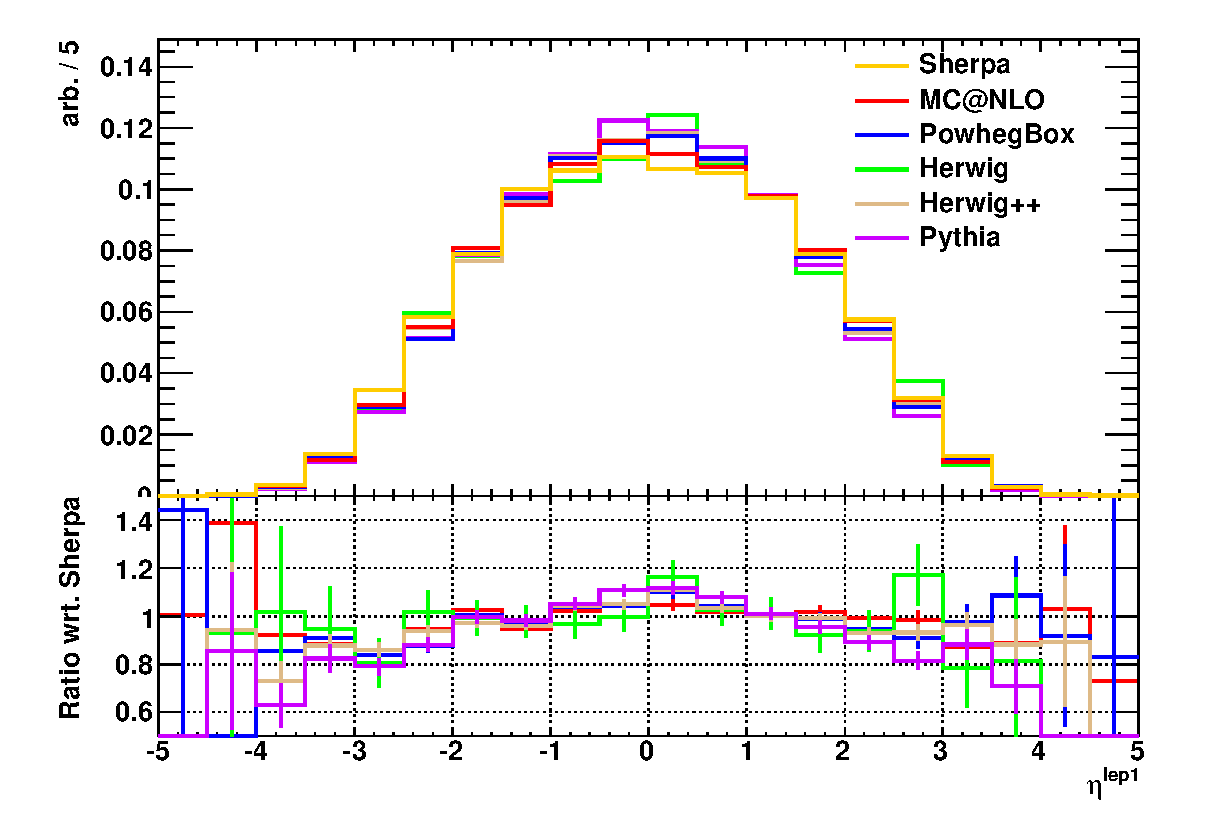
\includegraphics[width=0.47\textwidth]{GeneratorComparison/ZZ_lep_1_eta_2e2mu_wRatio_linear}
    }
        \vspace{-2mm}
    \subfigure[]{
        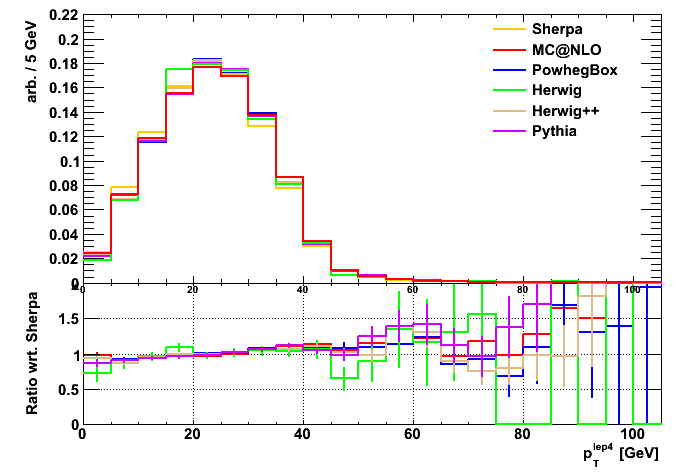
\includegraphics[width=0.47\textwidth]{GeneratorComparison/ZZ_lep_4_pt_2e2mu_wRatio_linear}
    }
    \subfigure[]{
        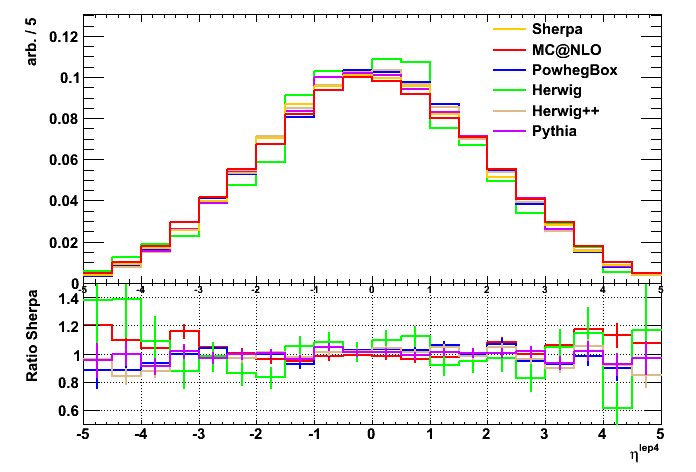
\includegraphics[width=0.47\textwidth]{GeneratorComparison/ZZ_lep_4_eta_2e2mu_wRatio_linear}
    }
        \vspace{-2mm}
    \caption{\small Comparison of generator level distributions, normalised to
    unit area, for \qqZZ $\ra\eemm$ as produced by different generators. Both 
    \Z\ bosons
    are required to have \sstooos. Figures (a)
    and (b) show the mass and \pt\ of the \ZZ\ system,
    respectively. Figures (c) and (d) show the \pt\ of the
    leading and subleading \Z, respectively. Figure (e) shows the \pt\ of the highest \pt\ lepton in the event, and figure (f) shows its
   $\eta$. Similarly figures (g) and (h) show the \pt\ and $\eta$ of the lowest
   \pt\ lepton in the event.}
    \label{fig:gen-comp-ZZ}
\end{figure}

%\begin{figure}
%\centering
%        \vspace{-5mm}
%    \subfigure[]{
%        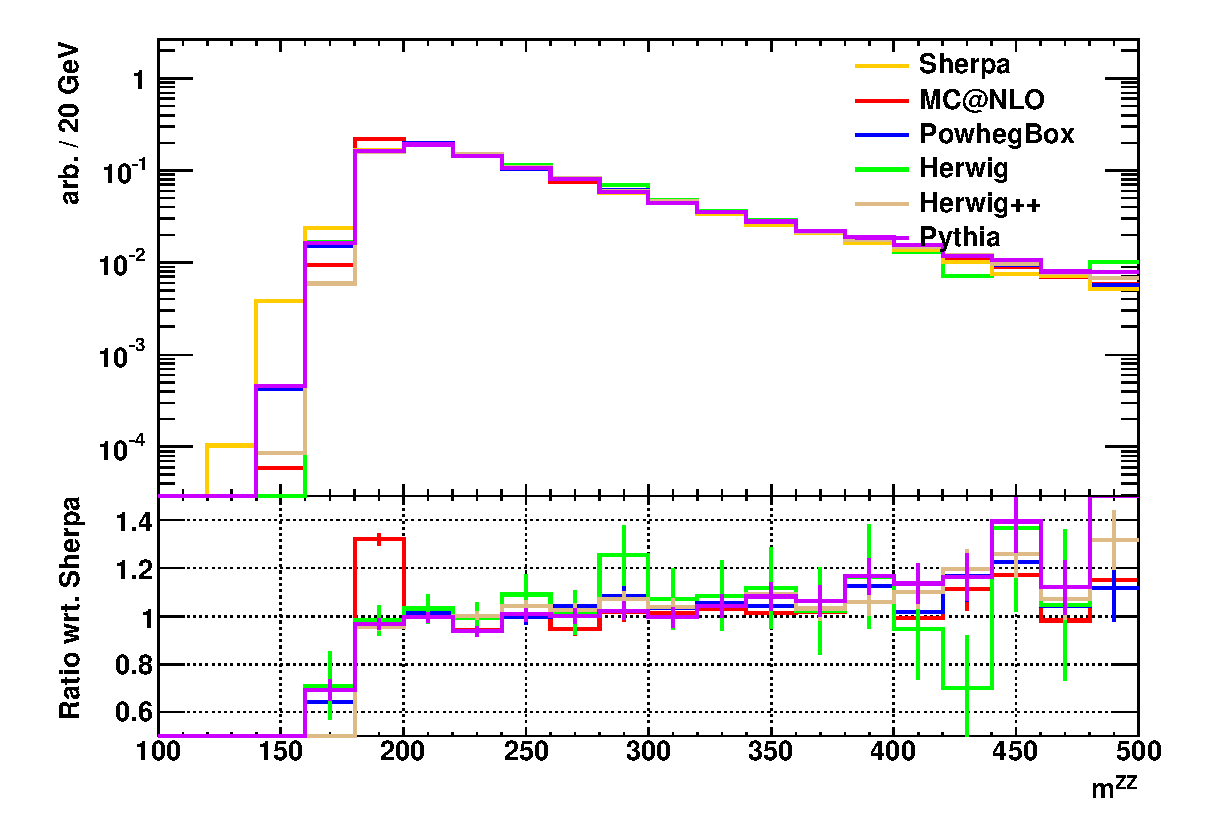
\includegraphics[width=0.47\textwidth]{GeneratorComparison/fidZZ_ZZ_m_2e2mu_wRatio_log}
%    }
%    \subfigure[]{
%        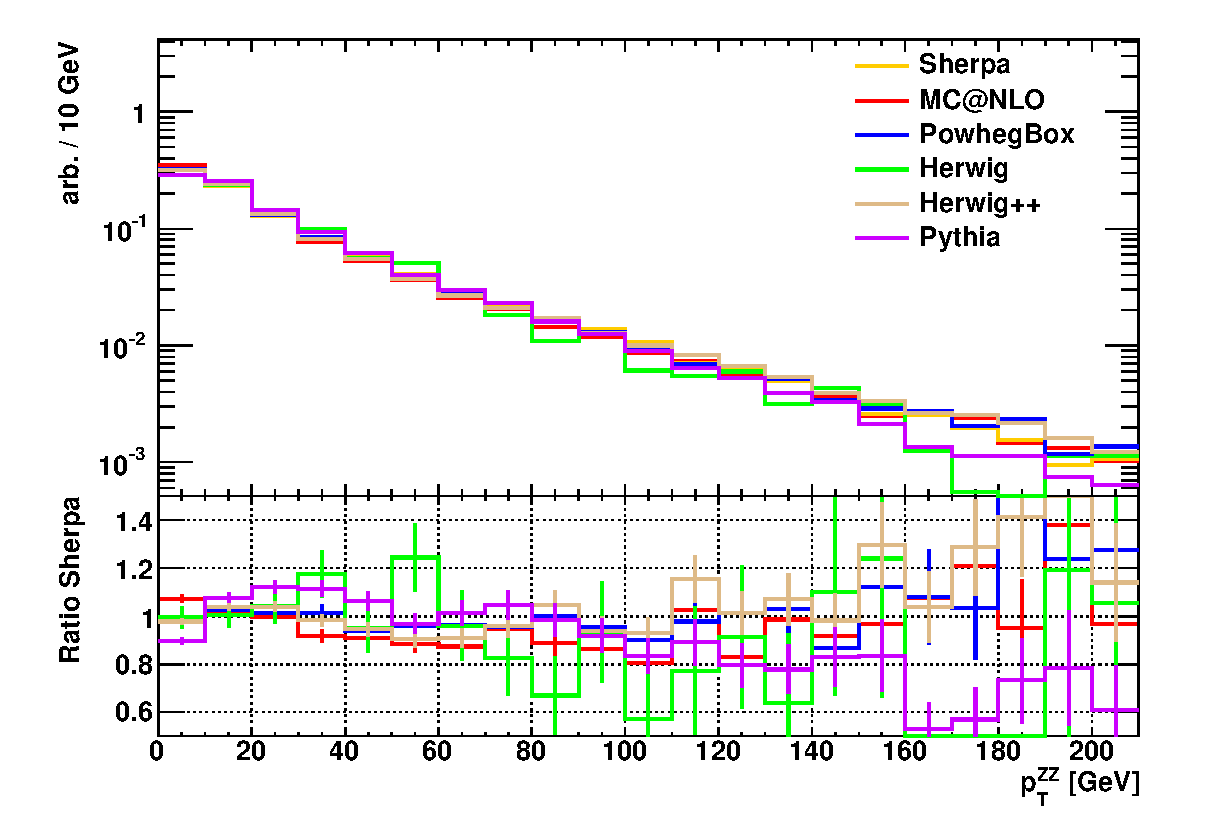
\includegraphics[width=0.47\textwidth]{GeneratorComparison/fidZZ_ZZ_pt_2e2mu_wRatio_log}
%    }
%        \vspace{-2mm}
%    \subfigure[]{
%        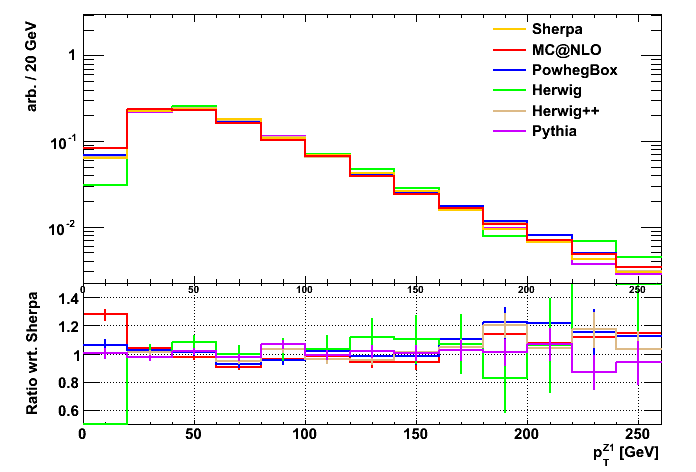
\includegraphics[width=0.47\textwidth]{GeneratorComparison/fidZZ_Z1_pt_2e2mu_wRatio_log}
%    }
%    \subfigure[]{
%        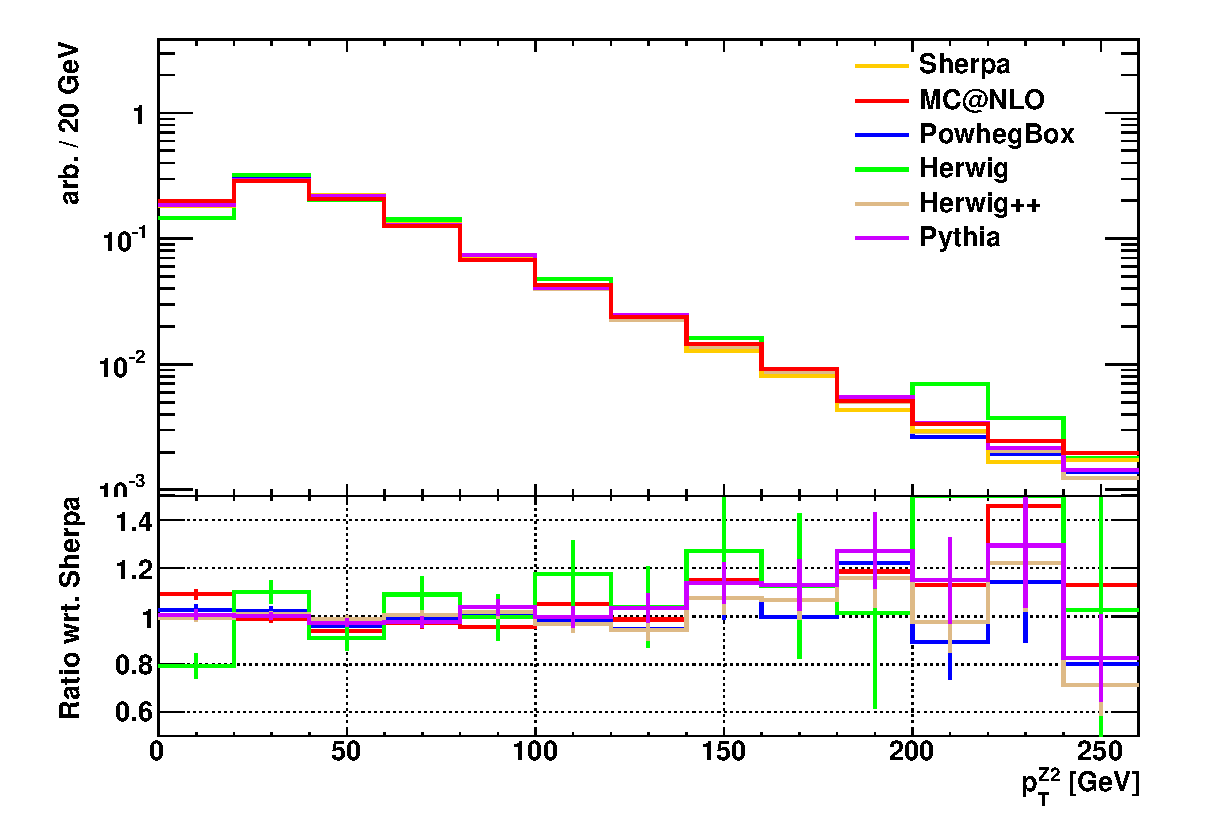
\includegraphics[width=0.47\textwidth]{GeneratorComparison/fidZZ_Z2_pt_2e2mu_wRatio_log}
%    }
%        \vspace{-2mm}
%    \subfigure[]{
%        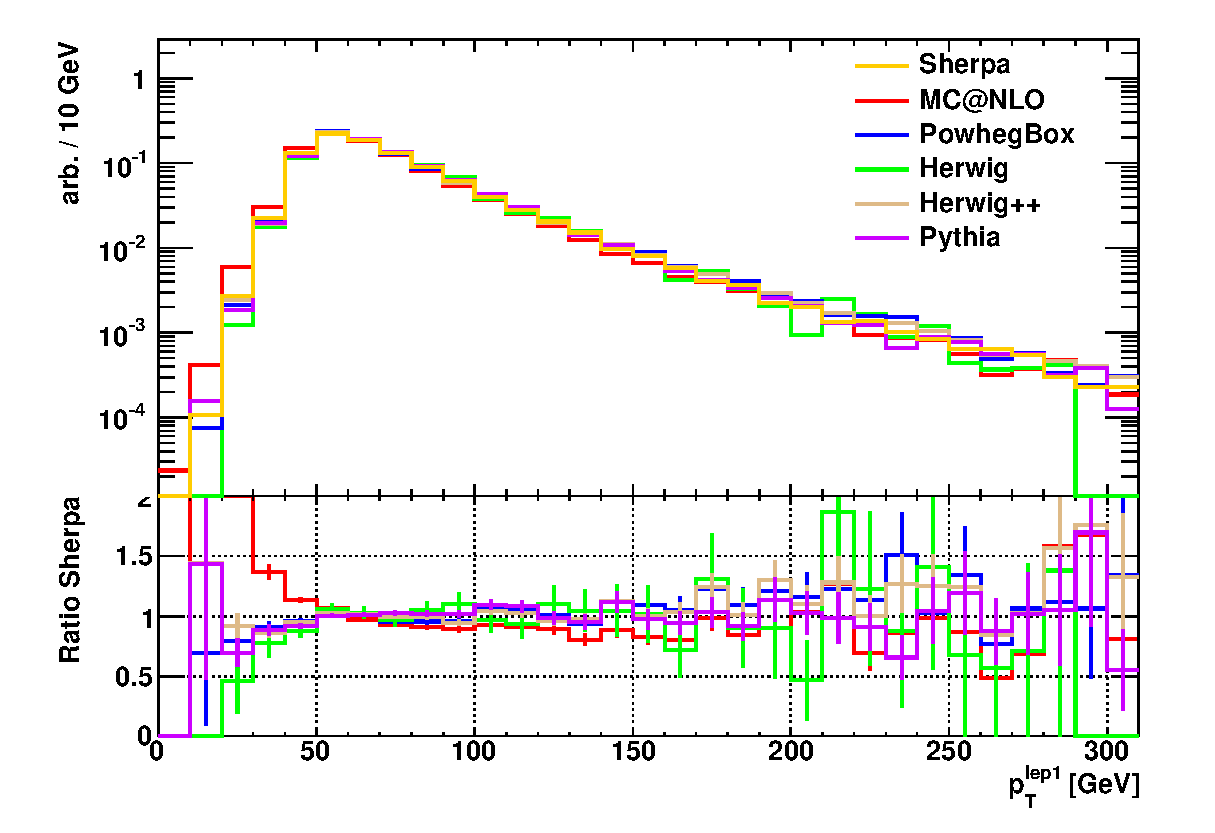
\includegraphics[width=0.47\textwidth]{GeneratorComparison/ZZ_lep_1_pt_2e2mu_wRatio_log}
%    }
%    \subfigure[]{
%        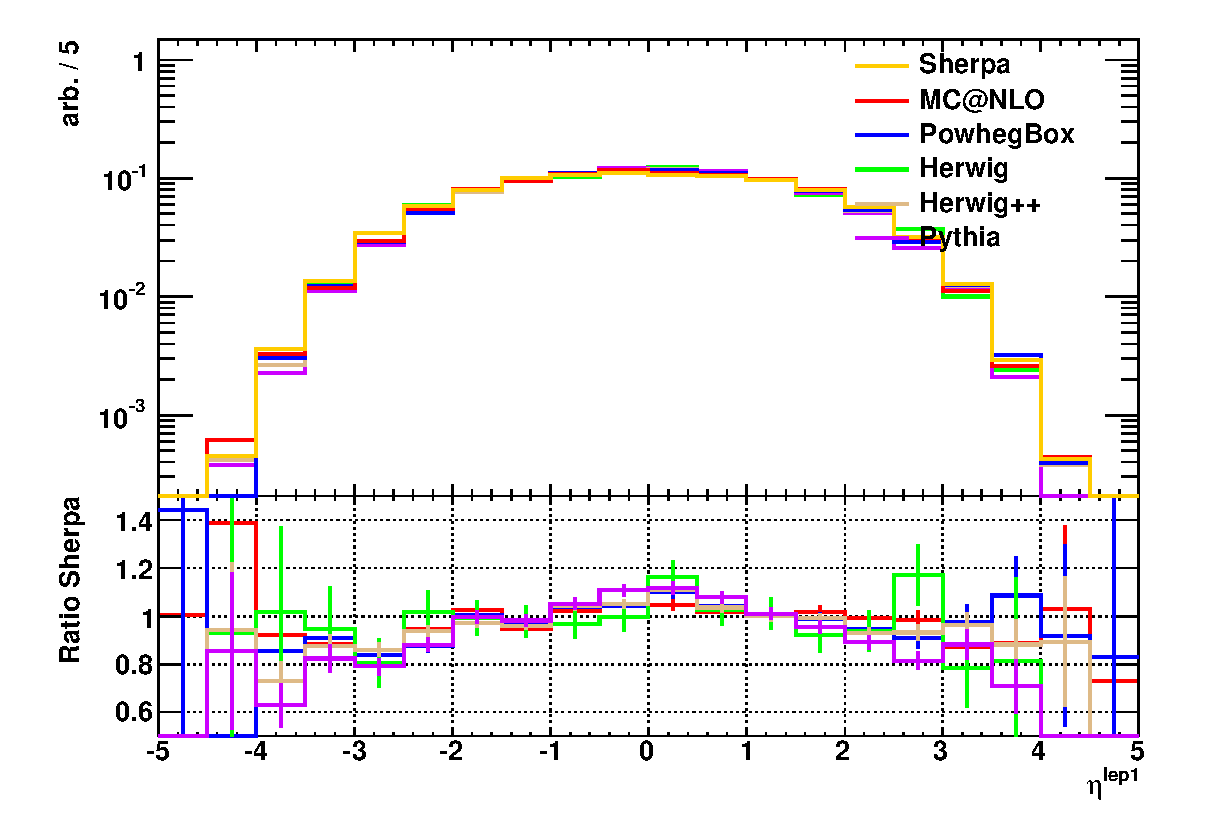
\includegraphics[width=0.47\textwidth]{GeneratorComparison/ZZ_lep_1_eta_2e2mu_wRatio_log}
%    }
%        \vspace{-2mm}
%    \subfigure[]{
%        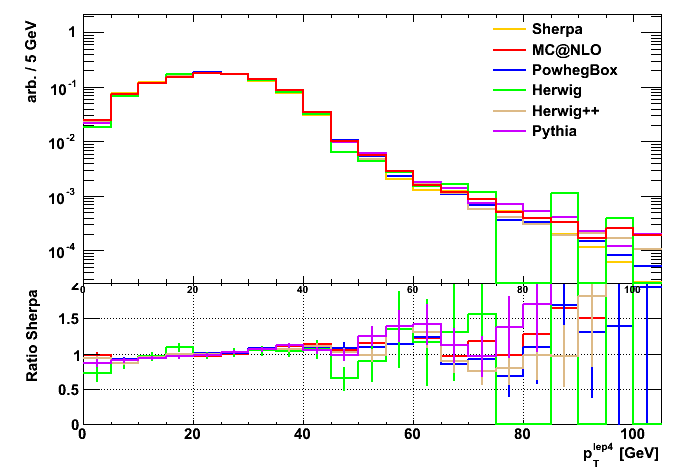
\includegraphics[width=0.47\textwidth]{GeneratorComparison/ZZ_lep_4_pt_2e2mu_wRatio_log}
%    }
%    \subfigure[]{
%        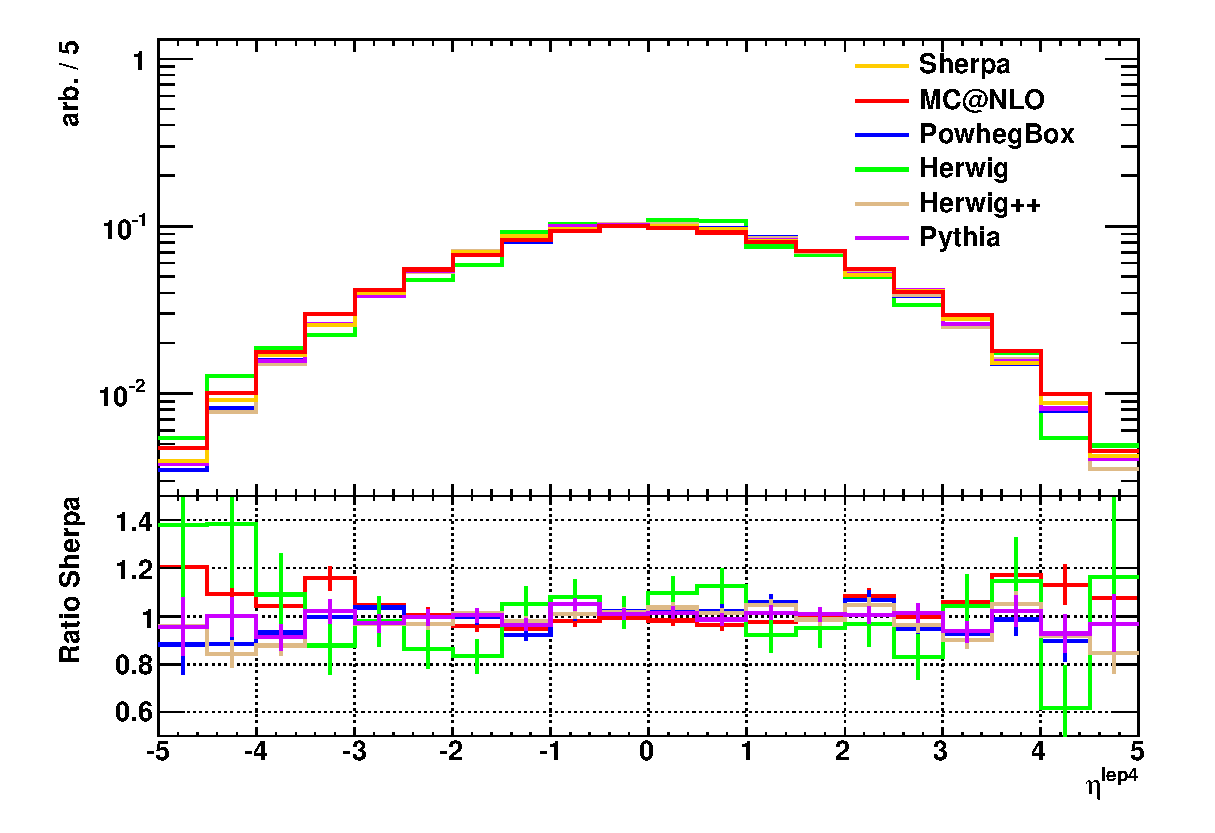
\includegraphics[width=0.47\textwidth]{GeneratorComparison/ZZ_lep_4_eta_2e2mu_wRatio_log}
%    }
%        \vspace{-2mm}
%    \caption{\small Comparison of generator level distributions, normalised to
%    unit area, for \ZZsllll\ proceeding via $qq$ and $gg$ interactions. One \Z\ is required to have \sstooos\ and the other
%    $m_{Z}>20$ \gev. Figures (a)
%    and (b) show the mass and \pt\ of the \ZZ\ system,
%    respectively. Figures (c) and (d) show the \pt\ of the
%    leading and subleading \Z, respectively. Figure (e) shows the \pt\ of the highest \pt\ lepton in the event, and figure (f) shows its
%   $\eta$. Similarly figures (g) and (h) show the \pt\ and $\eta$ of the lowest
%   \pt\ lepton in the event.}
%    \label{fig:gen-comp-7-8-ZZs}
%\end{figure}

%\begin{figure}
%\centering
%        \vspace{-5mm}
%    \subfigure[]{
%        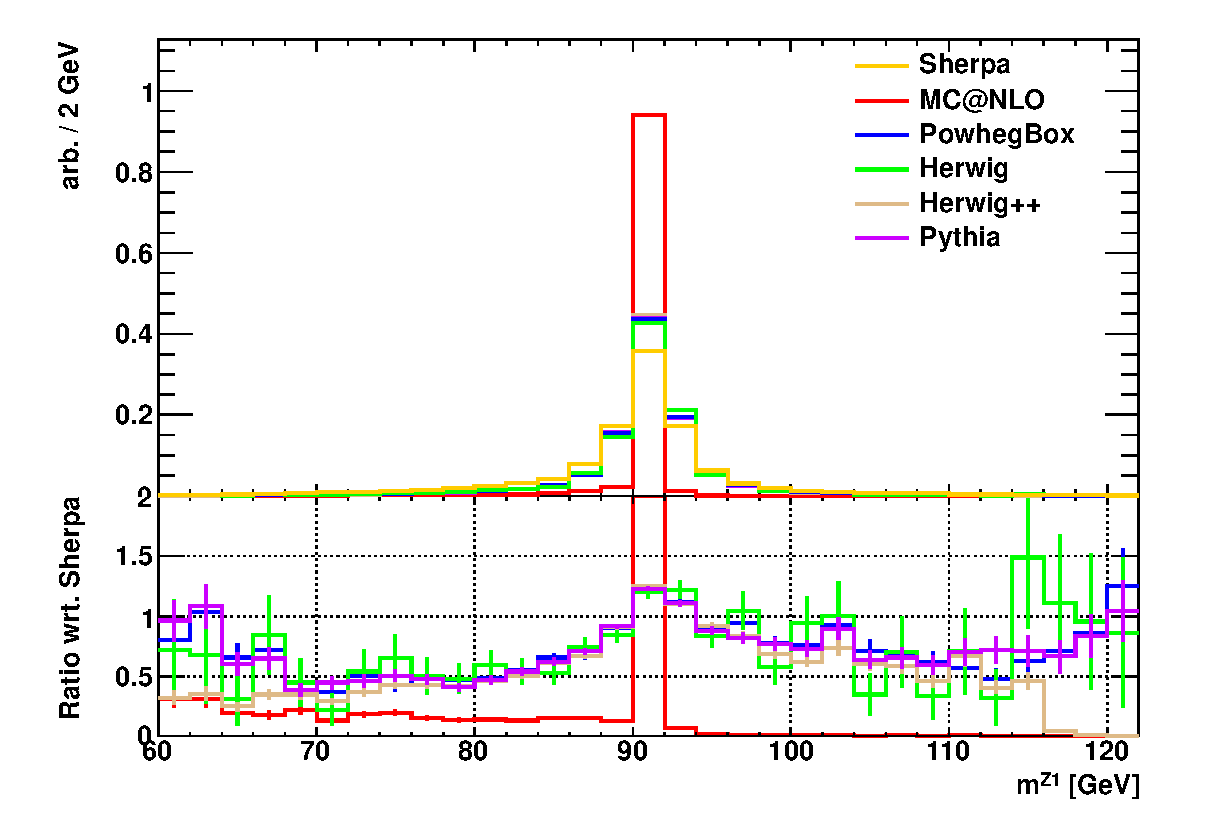
\includegraphics[width=0.47\textwidth]{GeneratorComparison/lepFid_Z1_m_nm1_2e2mu_wRatio_linear}
%    }
%    \subfigure[]{
%        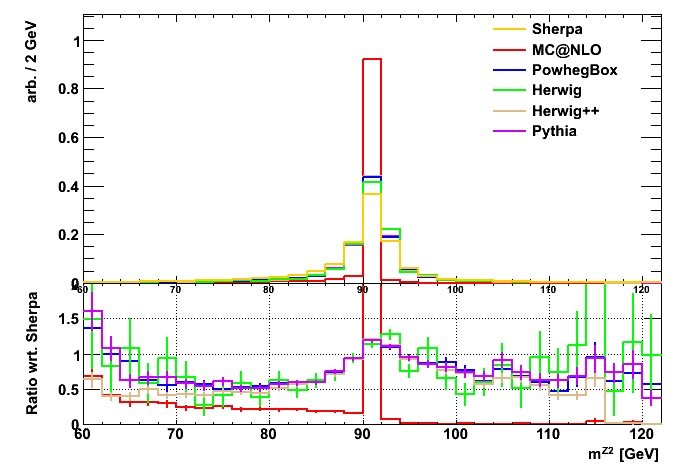
\includegraphics[width=0.47\textwidth]{GeneratorComparison/lepFid_Z2_m_nm1_2e2mu_wRatio_linear}
%    }
%        \vspace{-2mm}
%    \caption{\small Comparison of generator level distributions, normalised to
%    unit area, for \ZZsllll\ proceeding via $qq$ and $gg$ interactions. One \Z\ is required to have \sstooos\ and the other
%    $m_{Z}>20$ \gev. Figures (a)
%    and (b) show the mass and \pt\ of the \ZZ\ system,
%    respectively. Figures (c) and (d) show the \pt\ of the
%    leading and subleading \Z, respectively. Figure (e) shows the \pt\ of the highest \pt\ lepton in the event, and figure (f) shows its
%   $\eta$. Similarly figures (g) and (h) show the \pt\ and $\eta$ of the lowest
%   \pt\ lepton in the event.}
%    \label{fig:gen-comp-7-8-ZZs}
%\end{figure}

\begin{figure}
\centering
        \vspace{-5mm}
    \subfigure[]{
        \includegraphics[width=0.7\textwidth]{GeneratorComparison/lepFid_Zee_m_nm1_2e2mu_wRatio_log}
    }
    \subfigure[]{
        \includegraphics[width=0.7\textwidth]{GeneratorComparison/lepFid_Zmm_m_nm1_2e2mu_wRatio_log}
    }
        \vspace{-2mm}
    \caption{\small Comparison of generator level distributions, normalised to
    unit area, for \qqZZ $\ra\eemm$ as produced by different generators. Both 
    \Z\ bosons
    are required to have \sstooos. Figure (a)
    shows the invariant mass distribution for the dielectron pair whilst Figure 
    (b) shows the invariant distribution for the dimuon pair.
    } 
    
    \label{fig:gen-comp-mZ} 
    \end{figure}

\begin{figure}
\centering
        \vspace{-5mm}
    \subfigure[]{
        \includegraphics[width=0.7\textwidth]{SherpaQED/lepFid_Zee_m_nm1_2e2mu_wRatio_log}
    }
    \subfigure[]{
        \includegraphics[width=0.7\textwidth]{SherpaQED/lepFid_Zmm_m_nm1_2e2mu_wRatio_log}
    }
        \vspace{-2mm}
    \caption{\small \small Generator level \mZ\ distributions,
    comparing the distributions obtained from \sherpa\ by applying the QED
    radiation from the full $llll$ multipole (labelled $(llll)$), and assuming two
    separate dipoles, $\Z[\ell\ell]$ and $\Z[\ell'\ell']$ and radiating from
    them (labelled $(ll)(ll)$). The distribution from \powhegbox, which uses the
    second approach, is also shown for comparison. All distributions are
    normalised to unit area, and both \Z\ bosons are required to have \sstooos. Figure (a)
    shows the invariant mass distribution for the dielectron pair whilst Figure 
    (b) shows the invariant distribution for the dimuon pair.
}
    \label{fig:gen-comp-SherpaQED}
\end{figure}


%% TGC diagram
%\begin{figure}
%\centering
%        \vspace{10mm}
%    \mbox{
%    \subfigure{
%        \begin{fmffile}{schan}
%        \begin{fmfgraph*}(36,20)
%            \fmfleft{i1,i2}
%        \fmfright{o1,o2}
%        \fmflabel{$u,d$}{i2}
%        \fmflabel{$\bar{u},\bar{d}$}{i1}
%        \fmfright{o1,o2}
%        \fmflabel{$Z/\gamma^{*}$}{o1}
%        \fmflabel{$Z/\gamma^{*}$}{o2}
%        \fmf{fermion}{i2,v1,i1}
%        %\fmf{fermion}{v2,i2}
%        %\fmf{fermion}{v1,i1}
%        \fmf{photon,label=$Z/\gamma^{*}$}{v1,v2}
%        \fmf{photon}{v2,o1}
%        \fmf{photon}{v2,o2}
%        % uncommment this line if you want dots at the vertices
%            %\fmfdotn{v}{4}
%        \end{fmfgraph*}
%        \end{fmffile}
%    }
%    }
%        \vspace{5mm}
%    \caption{A diagram!}
%\end{figure}

Figures~\figure{fig:gen-comp-ZZ} and~\figure{fig:gen-comp-mZ} shows a comparison of kinematic distributions in \qqZZ
%$\ra\eemm$ 
vents generated using different \mc\ generators. The generators compared are
%\sherpa, \mcatnlo, \powhegbox, \herwig, \herwigPP\ and \pythia; descriptions of
%these generators are given in~\sec{Theory-MC-gen}. In all figures both \Z\
%bosons are required to have have \sstooos. 
%~\fig{gen-comp-mZ} shows the invarient mass distribution of the di-electron and
%di-muon pairs. Good agreement is seen between the different generators, with
%the exception of \mcatnlo, which uses a zero-width approximation for the \Z\
%bosons, and \sherpa, which is seen to have a slightly wider \Z\ lineshape.

The difference in the \Z\ line-shape observed between \sherpa\ and the other
generators is attributed to the fact that \sherpa\ applies QED FSR in a
different way. For all of the other generators compared in~\fig{gen-comp-mZ}, 
\photos~\cite{Golonka:2005pn} is used
to model QED radiation, whereas \sherpa\ has it's own internal treatment. There are two
ways of applying QED radiation to a \ZZllll\ final state. The radiation can
either be applied from the full $lll$\ multipole, distributing the recoil within
the multipole, or assuming two separate dipoles, $\Z[\ell\ell]$ and
$\Z[\ell'\ell']$, each
of which undergoes QED radiation independently from each other. The latter
treatment leaves the mass of each dilepton pair invariant, whereas the former
treatment leaves the mass of the four-lepton system invariant. \photos\ uses the
$(\ell\ell)(\ell'\ell')$ approach, whilst the \sherpa\ samples used in
~\fig{gen-comp-mZ}
use the $(llll)$ approach. ~\fig{gen-comp-SherpaQED} shows the difference 
between the \Z\
lineshape in \sherpa\ samples generated using the two approaches; the \Z\
lineshape in \sherpa\ samples generated using the $(\ell\ell)(\ell'\ell')$ approach agree with the productions from the generators using \photos. It is not  clear which is the correct approach
theoretically~\cite{Siegert}, so additional systematics are assigned to account
for differences resulting from the two approaches.

\section{Anomalous Triple Gauge Couplings}
Non-zero nTGCs would manifest as an increased \ZZ\
production \cx, especially at high \ZZ\ invariant mass and transverse
momentum~\cite{Baur:2000ae}.

%\section{ZZ Resonances}

%
\section{Previous experimental results}

Diboson ZZ production was first observed in $e^+e^-$ collisions at LEP in 1997
when the centre of mass energy of the collider first reached 183 \gev, the
threshold for producing two on-shell \Z\ bosons.
The L3 experiment published the first observation and \cx\ measurement
of on-shell \ZZ\ production~\cite{Acciarri1999281}, based on 55.3~\ipb\
of data collected at an average centre-of-mass energy of 182.7 GeV. All visible
decay-channels were used in the measurement. Whilst no events were
observed in the \llll\ final state, a total of 63 were observed in
the other visible final states. The majority (47) of these were in the
all-hadronic channel, which suffered from high backgrounds from $e^+e-
\rightarrow qq \gamma$ and $e^+e- \rightarrow WW$. In this channel a neural
network method was used to distinguish the signal events from the background. A
log-likelihood fit of the neural network output and the observed mass spectra in
the other channels was used to combine the channels, and gave a \cx\ of
$\sigma_{ZZ} = 0.30^{+0.22 +0.07}_{-0.16 -0.03}$, in very good agreement with
the \sm\ prediction. 

Measurements of the \ZZ\ production \cx\ in $e^+e^-$ collisions have
been made by all four LEP experiments at centre of mass energies between 183
\gev\ and 209
\gev~\cite{Abbiendi:2003va,Abdallah:2003dv,Acciarri:1999ug,Schael:1166743}.
These have been combined at each centre of mass energy using a \chisquared\
minimisation technique, taking into account correlations between the systematic
uncertainties~\cite{bib:LEPEW2006}. The resulting combined \cx s as a
function of centre of mass energy are shown in~\fig{lep-cx} and are in good agreement with
theoretical predictions.

\begin{figure}
\centering
        \includegraphics[width=0.7\textwidth]{lep_cx}
    \caption{Measurements of the \ZZ\ production \cx\ in  $e^+e^-$
    collisions as a function of centre of mass energy $\sqrt{s}$. The
    measurements are a combination of measurements from the four LEP
    experiments. Figure from~\cite{bib:LEPEW2006}.}
    \label{fig:lep-cx}
\end{figure}

Each of the LEP experiments also set limits on the \ZZZ\ and \ZZg\ anomalous
triple gauge couplings $f_{i}^{V}$. The limits are set using the measured total
\ZZ\ \cx, as well as kinematic distributions sensitive to to aTGCs.
ALEPH~\cite{Schael:1166743}, DELPHI~\cite{Bambade:1002930} and
OPAL~\cite{Abbiendi:2000kq} use the $\cos(\theta_{Z})$ distribution, where
$\theta_{Z}$ is the production angle of the \Z\ boson with respect to the beam
axis. L3~\cite{Acciarri:1999ug} use fits to different kinematic variables in
each decay channel. Each experiment first combines its limits across the different
decay channels and centre of mass energies, and provides the negative
log-likelihood as a function of the parameter to be combined. Limits are set
varying each parameter independently, holding the other parameters at their
standard model value of zero. Two parameter
fits are also carried out. No deviations from the \sm\ are observed. The
negative log-likelihood distributions from each of the experiments, as well as the
combined negative log-likelihood, are shown in~\fig{lep-tgc}, and the single
parameter limts are given in~\tab{prev-tgc-limits}.

\begin{figure}
\centering
        \includegraphics[width=0.7\textwidth]{lep_tgc}
    \caption{Negative log-likelihood curves for aTGC couplings from the four LEP
    experiments (coloured bands) and their combination (black band). Figure from~\cite{bib:LEPEW2006}.}
    \label{fig:lep-tgc}
\end{figure}

Measurements of the \ZZ\ production \cx\ in $p \bar{p}$
collisions at a centre of mass energy of $\sqrt{s} = 1.96$ \tev\ have been made
at the Tevatron by both the D0 and the CDF experiment. D0 measured the \ZZ\ \cx\ in
6.4~\ifb\ of integrated luminosity using the \ZZllll\
channel~\cite{Abazov:2011td} and in 8.6~\ifb\ using the
\ZZllvv\ channel~\cite{Abazov:2012cj}. In the \ZZllll\ channel 10 events
were observed with the requirement that both dilepon pairs have mass above 30
\gev, with an expected background of 0.37 $\pm$ 0.13. Combining the two
channels, the measured \cx\ for \ZZ\ production with the requirement of $60 < m_{\Z}
< 120$ \gev\ was 
\crossSec{p\bar p\ra ZZ}{\measStatSyst{1.44}{\errAsym{0.31}{0.28}}{\errAsym{0.17}{0.19}}~\rm{pb}}, 
in agreement with the \sm\ prediction of \crossSec{p\bar p\ra ZZ}{1.3 \pm 0.1 \, \rm{pb}}. 
The observed kinematic distributions were
also in good agreement with the \sm\ predictions. 

CDF~\cite{CDF:2011ab}
have measured the \ZZ\ \cx\ using the \ZZllvv\ and \ZZllll\
channels in 6 \ifb\ of integrated luminosity. In the \ZZllll\ channel, events
were required to have two \ossf\ lepton pairs, with one pair required to have
invariant mass within $\pm$ 25 \gev\ of the \Z\ mass, and the other in the range
$40 < m_{\ll} < 140$ \gev. 14 such events were observed, with an expect
background of 0.26\errAsym{0.53}{0.15} events. The measured \cx, combining the
two channels and correcting to the zero-width approximation, was \crossSec{p\bar
p\ra ZZ}{1.64\,\errAsym{0.44}{0.38}\, \rm{(stat+syst)\,pb}}, again in agreement with
the \sm\ prediction of \crossSec{p\bar p\ra ZZ}{1.4 \pm 0.1 \, \rm{pb}}.

Both experiments also set limits on aTGCs. D0 set limits using
\ZZllll\ decays in 1~\ifb\ of data~\cite{Abazov:2007ad}, requiring that
both dilepton pairs had an invariant mass $>$ 50 (70) GeV for dimuon (dielectron)
pairs. No events were observed passing this selection. 
Limits were set by comparing observed number of events with the yields predicted in
samples simulated with different values of the anomolous couplings.
 %this is used to form a likelihood for that point. 
 The resulting 95\% confidence limits obtained bu varying one
parameter at a time and holding the rest at zero are shown
in~\tab{prev-tgc-limits}. Two-dimenional limits were also
set.

%CDF search for anomolous couplings in the di-lepton di-jet final state.
% But the documentation is crap and data/MC agreement in CR is poor.
%http://www-cdf.fnal.gov/physics/ewk/2008/ZZZatGC/ZZZaTGC.html

Recently the CMS experiment have published a measurement of the \ZZ\ production
\cx\ in $pp$ collisions at 7~\tev~\cite{Chatrchyan:1495152} using
\ZZllll\ decays. In a dataset of 5 \ifb\ they select events with two \ossf\ dilepton
pairs, where the first dilepton pair must be composed of electrons or muons and
have a mass $60 < m_{\ll} < 120$ \gev. The second pair may be composed of either
electrons, muons or taus. In the case of the second pair being \ee\ or \mm\ the
same mass cut is applied as for the first pair. In the case of \tautau, the
visible mass is required to satisfy $30 < m_{\tau\tau}^{\rm{vis}} < 80$~\gev.
In the $4e$,$4\mu$ and $2e2\mu$ channels they observed 54 events, with a \sm\ prediction of
\measStatSyst{54.5}{\errSym{0.3}}{\errSym{4.8}} (including a small background
component). In the $2\ell2\tau$ channels,
11 events were observed, with a \sm\ prediction of
\measStatSyst{11.7}{\errSym{0.8}}{\errSym{1.0}} (including 4.4 from background
processes). Combining all final states, the measured \cx, requiring both \Z\
bosons to be in the range 60 $< m_{Z} < 120$ \gev, was found to be \crossSec{p
p\ra
ZZ}{\measStatSystLumi{6.24}{\errAsym{0.86}{0.80}}{\errAsym{0.41}{0.32}}{\errSym{0.14}}\,pb},
in excellent agreement with the \sm\ prediction of 6.3 \errSym{0.4}~pb. Limits
were set on aTGCs using the observed four-lepton mass distribution for the
$4e$,$4\mu$ and $2e2\mu$ channels combined. The observed 95\% confidence limits
on aTGCs from LEP, D0 and CMS are given in~\tab{prev-tgc-limits}.

\begin{table}[htbp]
\small
\begin{center}
\begin{tabular}{lccccc} \hline\hline
Experiment & $\Lambda, \, n$ & \ffourZ & \ffiveZ & \ffourg & \ffiveg \\
\hline
LEP & $\infty, -$ & [-0.30, 0.30] & [-0.34, 0.38]  & [-0.17, 0.19]   & [-0.32,
0.36] \\
D0 & 1.2 \gev, 3  & [-0.28, 0.28]  & [-0.31, 0.29]     &  [-0.26, 0.26]     &
[-0.30, 0.28] \\
CMS & $\infty, -$ & [-0.011, 0.012]  & [-0.012, 0.012]   & [-0.013, 0.015]  &
[-0.014, 0.014] \\
\hline\hline
\end{tabular}
\end{center}
\caption{95 \% confidence level limits on anomolous triple gauge coupling
parameters obtained from LEP~\cite{bib:LEPEW2006}, D0~\cite{Abazov:2007ad} and
CMS~\cite{Chatrchyan:1495152}. In each case the cutoff scale $\Lambda$ and form
factor $n$ is indicated.}
\label{table:prev-tgc-limits}
\end{table} 
